\chapter{Metodolog\'ia}

El capítulo anterior hace referencia a las teorías recientes que son
utilizados para la autonomía de un robot móvil y para la generación de
un mapa bidimensional, dentro de un ambiente aún por conocer. En el presente
trabajo de tesis se ha desarrollado un sistema de movimiento 
autónomo, del robot móvil, basado en campos potenciales, leyes de control 
polar y posiciones aleatorias dentro de un espacio de configuración. Este sistema
permite lograr que el robot pueda explorar un ambiente desconocido de manera
autónoma. Asimismo, también se ha desarrollado un sistema mecánico accionado 
por un motor paso a paso, el cual permite que el robot mientras se va desplazando
dentro de un entorno este pueda tomar mediciones en los tres ejes del plano
cartesiano y así obtener una representación gráfica del lugar en tres 
dimensiones. Estos sitemas pueden ser implementados desde una computadora en 
tiempo real (\textit{online}) o también puede ser implementado por medio de 
un microcontrolador (\textit{onboard}). En este capítulo se explicará, con 
detalles, los métodos que fueron implementados para realizar el presente trabajo.

%En el cap\'itulo anterior se explic\'o sobre las metodolog\'ias recientes que se 
%utilizan para que un robot pueda ser aut\'onomo y genere un mapa 
%del entorno donde se encuentre. En este trabajo de tesis se propone 
%el movimiento aut\'onomo basado en campos potenciales y en leyes de control 
%polar para el movimiento de un robot m\'ovil, de modo que sea capaz de alcanzar 
%un objetivo que vuelva a planificar continuamente su camino sin colisiones. El 
%algoritmo desarrollado puede ser implementado desde una computadora en tiempo 
%real (\textit{online}) o tambi\'en puede ser implementado por medio de un 
%microcontrolador (\textit{onboard}). En este cap\'itulo se explicar\'a, con detalles, 
%los m\'etodos que fueron implementados en este trabajo.

\section{Ejemplo de Aplicación}
En esta sección se explica sobre los componentes que fueron utilizados para construir
el prototipo funcional. Estos componentes se utilizan para la navegación 
autónoma del robot móvil, para construir el mapa en dos dimensiones y para tomar medidas 
en los tres ejes del plano cartesiano. Para la navegación se utilizó un robot móvil 
diferencial terrestre, y un sensor lidar para las mediciones del entorno.
%En esta secci\'on se explica cada uno de los componentes que tuvo que 
%ser utilizados para realizar la autonom\'ia y el mapeo de este trabajo de 
%tesis. Para realizar la autonom\'ia se utiliz\'o un robot m\'ovil diferencial 
%terrestre, y as\'i tambi\'en para mapear el entorno por donde el robot se 
%desplaza se utiliz\'o un sensor lidar.

%\subsection{Descripci\'on del Robot M\'ovil}
% \begin{figure}%[h]
% \centering \footnotesize
% {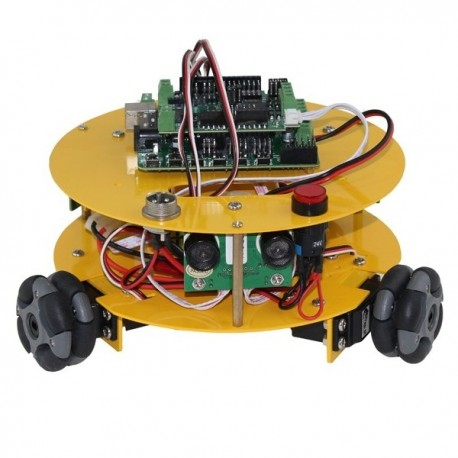
\includegraphics[width=0.40\linewidth]{images/omnidirecional.jpg}}
% \captionsetup{font=footnotesize}
% \caption{Robot m\'ovil hol\'onomico omnidireccional}
% \label{fig:omnidirectional}
% \end{figure}
% \begin{figure}%[h]
% \centering \footnotesize
% {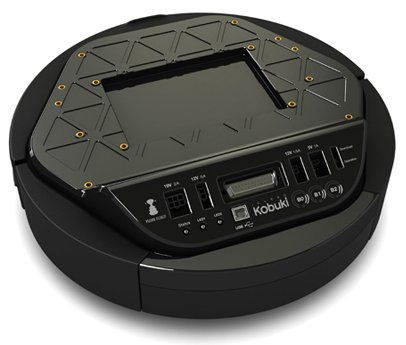
\includegraphics[width=0.40\linewidth]{images/kobuki.jpg}}
% \captionsetup{font=footnotesize}
% \caption{Robot m\'ovil no-hol\'onomico utilizado para implementar el 
% algoritmo de autonom\'ia}
% \label{fig:kobuki}
% \end{figure}
% Una forma de clasificar a los robots m\'oviles es a trav\'es de la locomoci\'on 
% de sus ruedas, esto se divide en dos: (1) robot holon\'omico y (2) robot 
% no-holon\'omico. El robot holon\'omico no tiene ninguna restricci\'on, con 
% respecto a la velocidad, en la posici\'on y la orientaci\'on. El robot se puede 
% mover instant\'aneamente en cualquier direcci\'on del espacio, sin necesidad de 
% rotar previamente. La mayor\'ia de estos robots m\'oviles son omnidireccionales, 
% como se puede ver en la figura \ref{fig:omnidirectional}. En cambio un robot 
% no-holonomico tiene una restricci\'on en su velocidad, no existe un trayectoria 
% que dependa solamente de la posici\'on y orientaci\'on. Por ende, este robot no 
% se puede mover instant\'aneamente en cada direcci\'on del espacio.

%Para este trabajo se hizo uso del robot m\'ovil no-holon\'omico, Kobuki (figura \ref{fig:kobuki})
%el cual esta configurado para poder trabajar con ROS (\textit{Robot Operating System}) 
%con una velocidad de translaci\'on de 70 $cm/s$, una velocidad de rotaci\'on de 180 
%$grados/s$, una posibilidad de carga de hasta 5 $kg$, un tiempo de operaci\'on de 3 
%horas \cite{aboutKobuki}. 

\subsection{Cinemática de Robot Móvil Diferencial}
\begin{figure}%[h]
\centering \footnotesize
{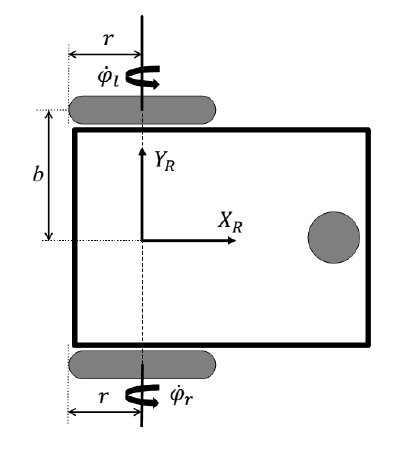
\includegraphics[width=0.40\linewidth]{images/kinematic_model.png}}
\captionsetup{font=footnotesize}
\caption{Representación gráfica de un robot móvil diferencial. Donde 
$b$ es la distancia de su centro de masa hacia sus ruedas, el radio de cada 
rueda es representado por $r$. Finalmente $\dot{\varphi_{l}}$ y 
$\dot{\varphi_{r}}$ son las velocidades de la rueda derecha y rueda izquierda 
correspondientemente.}
\label{fig:RMkinematic}
\end{figure}
La realización del modelo cinemático, del robot móvil diferencial, debe 
tener ciertas consideraciones con respecto a su comportamiento. Primero, 
se debe asumir que el robot se desplaza dentro de una superficie plana 
idealmente sin ningún tipo de rozamiento, y segundo se debe tomar los ejes
de las ruedas de forma perpendicular al suelo, existiendo un solo punto 
de contacto entre el suelo y la rueda.
%Para realizar el modelo cinemático del robot diferencial se debe tener 
%en cuenta algunas consideraciones sobre el comportamiento de este. Se asume 
%que el robot se desplaza en una superficie plana idealmente sin rozamiento, 
%también se toman los ejes de las ruedas como perpendiculares al suelo
%por donde se desplaza y que solo existe un punto de contacto entre 
%la rueda y el suelo.

%El robot se considera como un cuerpo r\'igido sin partes flexibles, pero se 
%deben tener en cuenta las restricciones no-holon\'omicas. Es decir, el robot 
%puede desplazarse hacia atr\'as o hacia adelante, pero no puede trasladarse 
%hacia los lados. Para poder realizar estos movimientos, se debe realizar un 
%movimiento en partes.

Para realizar las ecuaciones matemáticas del modelo cinemático del robot móvil, se
necesita conocer las dimensiones de este. Las medidas requeridas son el radio de las 
ruedas y la distancia entre cada una de ellas. El radio de las ruedas es representado
con la variable $r$ y la distancia entre ruedas es representada como $2b$. Otro punto 
a considerar es que el robot tiene dos ruedas convencionales fijas y el sistema de
referencia de este se encuentra en medio de las ruedas traseras, como se puede ver en 
la Figura \ref{fig:RMkinematic}.

%El modelo cinemático del robot necesita conocer las dimensiones del robot. Las 
%medidas que se necesitan son la distancia entre las ruedas y el radio de las 
%mismas. La distancia entre las ruedas es representada como $2b$ y el radio de 
%las ruedas como $r$. También se debe considerar que el robot tiene dos ruedas 
%convencionales fijas y el sistema de referencia del robot se encuentra entre 
%ambas ruedas, como se ve en la Figura \ref{fig:RMkinematic}.

Teniendo en consideración las restricciones de las ruedas convencionales se halla la 
cinemática directa del robot móvil. La cinemática directa consiste en:
\begin{align*}
v &= \frac{r}{2}(\dot{\varphi_{r}} + \dot{\varphi_{l}}), \\
\omega &= \frac{r}{2b}(\dot{\varphi_{r}} + \dot{\varphi_{l}}),
\end{align*}
donde $v$ es la velocidad lineal y $\omega$ es la velocidad angular. Estas 
dos variables de velocidad se pueden hallar a través de las velocidades
de cada una de las ruedas y las dimensiones del robot. Por otro lado la cinemática 
inversa, como su mismo nombre lo menciona, es todo lo contrario a la
cinemática directa y consiste en: 
\begin{align*}
\dot{\varphi_{r}} &= \frac{1}{r}(v + b\omega), \\
\dot{\varphi_{l}} &= \frac{1}{r}(v - b\omega),
\end{align*}
donde se halla las velocidades de las ruedas a partir de la velocidad lineal y velocidad
angular del robot móvil.
\begin{figure}%[h]
 \centering \footnotesize
 %{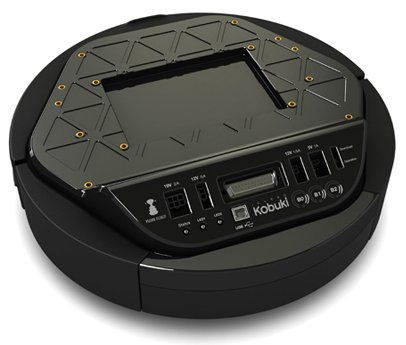
\includegraphics[width=0.35\linewidth]{images/kobuki.jpg}}
 {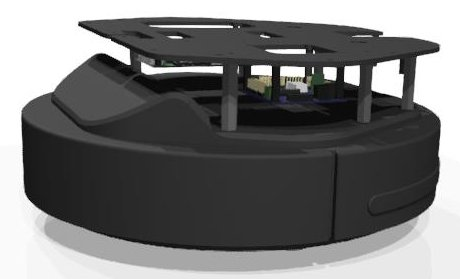
\includegraphics[width=0.35\linewidth]{images/turtlebot.jpg}}
 \captionsetup{font=footnotesize}
 \caption{Representación gráfica del robot móvil diferencial utilizado para la implementación 
 del sistema de navegación aútonoma.}
 \label{fig:kobuki}
 \end{figure}

Finalmente, para este trabajo de tesis se utilizó un robot móvil no-holonómico llamado Kobuki 
(ver Figura \ref{fig:kobuki}). Este robot trabaja con una velocidad de translación de 70 $cm/s$ y 
una velocidad de rotación de 180 $grados/s$. Tiene una posibilidad de carga de hasta 5 $kg$ y un 
tiempo de operación de 3 horas \cite{aboutKobuki}. En este robot se implementó las ecuaciones 
de la cinemática directa teniendo en consideración sus propias dimensiones y asimismo, haciendo
uso de las librerías que existe dentro de los paquetes de desarrollo del robot Kobuki.
%Para calcular la cinem\'atica del robot m\'ovil se debe usar las restricciones 
%de las ruedas convencionales. Las restricciones de cada rueda fija son:
%\begin{equation*}
%\[-\text{sin}(\alpha + \beta) & \text{cos}(\alpha + \beta) & \text{lcos}(\beta)\] 
%{R}^R_{I} {I}^\dot{\xi} - r\dot{\varphi} &= 0 \\
%\[\text{cos}(\alpha + \beta) & \text{sin}(\alpha + \beta) & \text{lsin}(\beta)\]
%{R}^R_{I} {I}^\dot{\xi} &= 0
%\end{equation}
%donde ${R}^R_{I}$ es la matriz de rotaci\'on que lleva el sistema de coordenadas del 
%robot $(X_{R},Y_{R})$ al sistema inercial $(X_{I},Y_{I})$ y $\dot{\xi}$ 
%es el vector que contiene los valores de las velocidades lineales y angular 
%del robot.


\subsection{Sistema de Percepción Bidimensional}
\begin{figure}%[h]
	\centering \footnotesize
 	{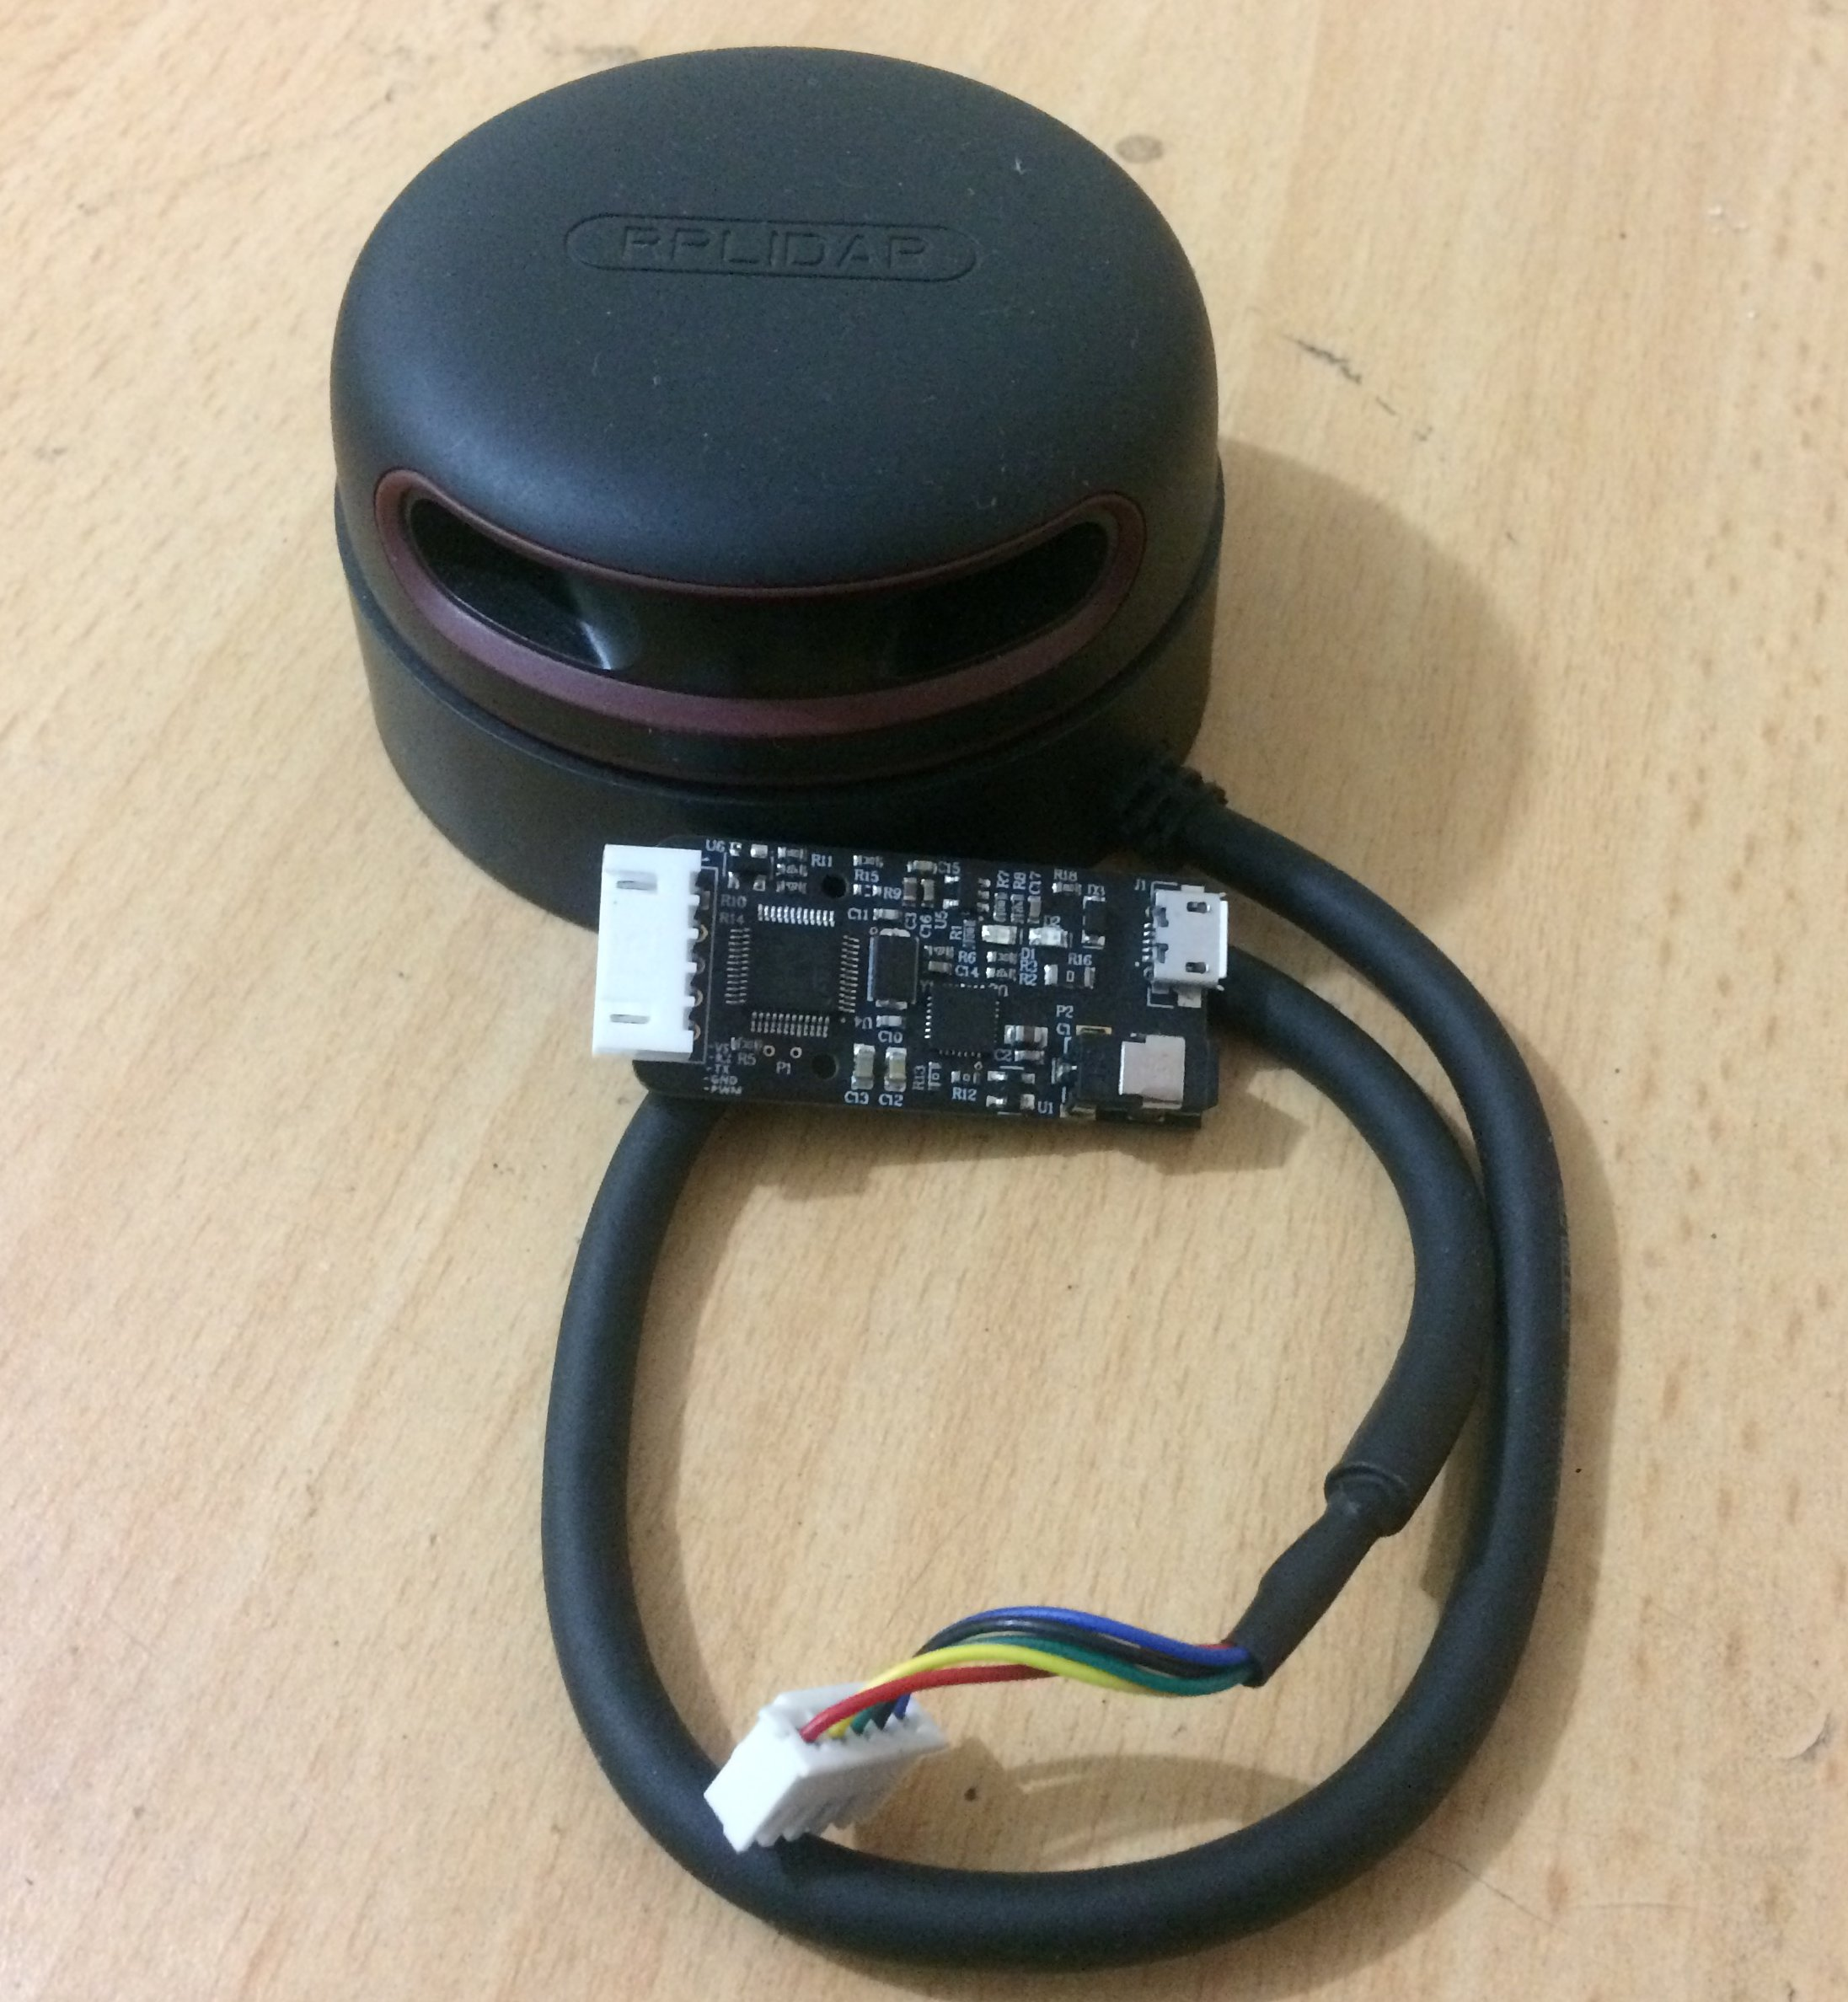
\includegraphics[width=0.60\linewidth]{images/rplidar.JPG}}
 	\captionsetup{font=footnotesize}
 	\caption[Sensor lidar RPLIDAR A2.]{Sensor lidar RPLIDAR A2 \cite{sensorLidar}.}
 	\label{f:lidar}
\end{figure}

Para generar un mapa de dos dimensiones dentro de un entorno, se necesita realizar 
mediciones dentro del ambiente. En este trabajo de tesis se utiliza un sensor lidar
llamado RPLidar A2, el cual se basa en el principio de rango de triagulación láser
\cite{amann2001laser}. Este sensor fue desarrollado por la empresa \textit{SLAMTEC}.

%Para generar el mapa de un entorno, se necesita medir distancias del ambiente y así
%generar el mapa. En este trabajo se utiliza un sensor lidar, RPLidar A2, el cual se basa en 
%el principio de rango de triangulación láser \cite{amann2001laser} y ha sido desarrollado 
%por la empresa \textit{SLAMTEC}.

El RPLidar A2 es un sensor que no necesita tener una luz externa para poder obtener las
medidas de las distancias. Este sensor tiene un láser infrarrojo de baja potencia el cual
es controlado por medio de un pulso modulado. Este sensor puede girar en 360\grad ~y tiene
un rango de alcance máximo de 6 metros. Trabaja a una frecuencia de 10Hz teniendo una tasa 
de medición de 4000 muestras por segundo. La transmisión de datos de este sensor es por 
medio de un protocolo UART. El sensor es mostrado en la Figura \ref{f:lidar}.


%Es un sensor l\'aser que se basa en el  principio de rango de triangulaci\'on 
%láser \cite{amann2001laser} y adopta el hardware de adquisici\'on y 
%procesamiento de visi\'on de alta velocidad desarrollado por \textit{SLAMTEC}. El 
%sensor utiliza un l\'aser infrarrojo de baja potencia como su fuente de luz y lo 
%maneja utilizando un pulso modulado. Este sensor gira a 360 \grad ~y llega a 
%una distancia m\'axima de 8 metros. Trabaja a una frecuencia de 10 Hz y 
%tiene una tasa de medici\'on de 4000 muestras por segundo. El hardware del 
%RPLIDAR A2 se puede ver en la figura \ref{f:lidar}, el cual tiene un 
%convertidor de protocolo UART a mini USB.


\begin{table}[htbp]
\begin{center}
\begin{tabular}{|l|c|c|c|c|}
	\hline
	Item & Unidad & M\'inimo & T\'ipico & M\'aximo\\
	\hline \hline
	Rango de distancia & m & 0.15 & - & 6 \\ \hline
	Rango angular & grados & - & 0 - 360 & - \\ \hline
	Resoluci\'on de la distancia & mm & - & menor a 0.5 & - \\ \hline
	Duraci\'on de muestra & ms & - & 0.25 & - \\ \hline
	Resoluci\'on angular & grados & 0.45 & 0.9 & 1.35 \\ \hline
	Fecuencia de muestreo & Hz & 2000 & 4000 & 4100 \\ \hline
	Frecuencia de escaneo & Hz & 5 & 10 & 15 \\ \hline
\end{tabular}
	\caption{Pruebas de Medici\'on del sensor RPLidar A2.}
	\label{tbl:medicion}
\end{center}
\end{table}

En la Tabla \ref{tbl:medicion} se muestra el rendimiento de la medición del 
sensor RPLidar A2 \cite{Slamtec}. En esta tabla se considera varias pruebas 
por cada una de las variables. Las variables más importantes son: (i) 
\textbf{Rango de distancia}, el sensor tiene un rango de medición entre $0.15 
m$ y $6 m$, los valores menores a $0.15 m$ y mayores a $6 m$ son 
considerados como valores no existentes. (ii) \textbf{Resolución de la 
distancia}, el sensor tiene un error menor a 0.5 $mm$ en sus mediciones, esto 
permite construir un mapa con las dimensiones reales del entorno. (iii) 
\textbf{Resolución angular}, este sensor tiene una resolución de 1\grad~ esto 
quiere decir que por cada grado que gira el sensor lidar este realiza una medición, 
por lo tanto el sensor toma 360 mediciones por cada rotación.
%La Tabla \ref{tbl:medicion} muestra el rendimiento de medición del 
%sensor lidar \cite{Slamtec} considerando varias pruebas por cada variable. Las variables más 
%importantes de esta Tabla son: (i) Rango de distancia, el sensor toma mediciones en el
%rango mostrado, cuando la distancia es menor a 0.15 $mts$ no considera la medición, lo 
%mismo sucede cuando la medición es mayor a 8 $mts$. (ii) Resolución de la distancia, el 
%sensor tiene un error menor a 0.5 $mm$ en sus mediciones, esto permite construir un mapa 
%con las dimensiones reales del entorno.(iii) Resolución angular, este sensor tiene una 
%resolución de 1\grad~ esto quiere decir que por cada grado que gira el lidar esta realizando 
%una medición, por lo tanto el sensor mide 360 veces por cada rotación.

\begin{figure}
	\centering \footnotesize
	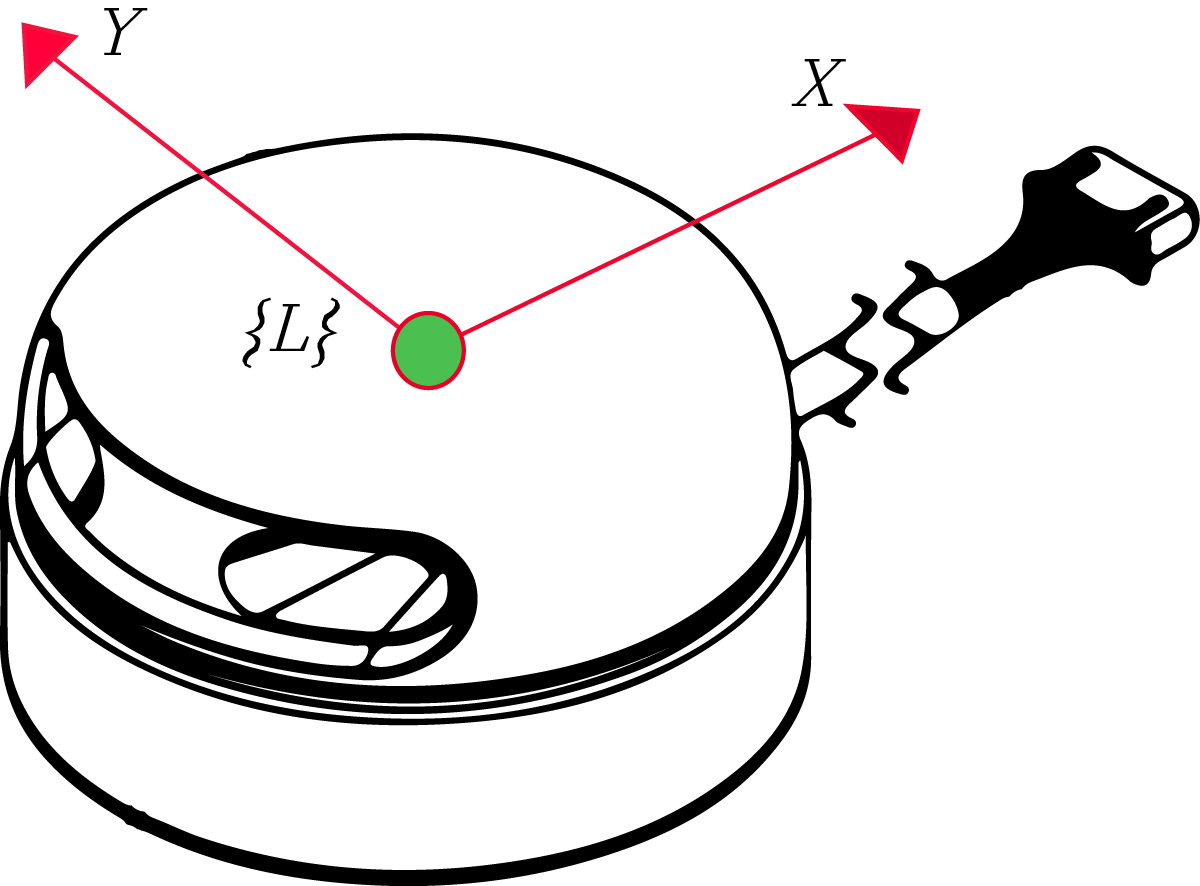
\includegraphics[width=0.40\linewidth]{images/frame_laser.png}
	\captionsetup{font=footnotesize}
	\caption{En esta figura el punto verde representa el sistema de referencia 
	del sensor RPLidar A2, donde el eje $\mayusx$ va en el mismo sentido del cable 
	de datos del sensor lidar.}
	%\caption{Sistema de referencia del sensor RPLidar A2.}
	\label{fig:FrameLidar}
\end{figure}

Para envíar los datos, a la computadora o al microcontrolador, el sensor trabaja con un 
protocolo de comunicación UART (\textit{Universal Asynchronous Receiver-Transmitter}). Este 
protocolo se especifíca en la Tabla \ref{tbl:comunicacion}, y a través del protocolo se 
obtiene las mediciones del sensor. Para la construcción del mapa en dos dimensiones se 
debe considerar el sistema de referencia del sensor lidar. En la Figura \ref{fig:FrameLidar} 
se muestra que el cable de comunicación indica la dirección y posición del eje $\mayusx$, al 
lado derecho se muestra la dirección y posición del eje $\mayusy$. Teniendo en cuenta la 
posición del sistema de referencia del sensor lidar, se puede comenzar a tomar los datos de 
las mediciones que va realizando. El sensor lidar envía como datos la distancia de la medición y 
el ángulo donde se tomo la medición. Estos datos obtenidos son tomados como coordenadas polares 
los cuales son convertidos a coordenadas cartesianas, de esta forma estimamos las posiciones de 
los objetos que se encuentran dentro de un ambiente.

%Para construir el mapa en dos dimensiones se tiene que tomar en 
%consideración el sistema de referencia del sensor lidar. En la Figura \ref{fig:FrameLidar} se 
%puede ver que el cable de comunicación indica la dirección del eje $\mayusx$ y al lado derecho 
%se encuentra posicionado el eje $\mayusy$. Teniendo en consideración el sistema de referencia 
%del sensor se puede obtener las distancias del entorno que se esta midiendo y a partir de una 
%conversión de coordenadas polares a coordenadas cartesianas se estima las posiciones de los objetos 
%que se encuentran dentro del entorno de trabajo.

\begin{table}[htbp]
\begin{center}
\begin{tabular}{|c|c|c|c|c|c|}
	\hline
	Color & Nombre de la señal & Tipo & Mínimo & Típico & Máximo \\ 
	\hline \hline
	Rojo & VCC & Potencia & 4.9V & 5V & 5.5V \\ \hline
	Amarillo & Tx & Salida & 0V & 3.3V & 3.5V \\ \hline
	Verde & Rx & Entrada & 0V & 3.3V & 3.5V \\ \hline
	Negro & GND & Potencia & 0V & 0V & 0V \\ \hline
	Azul & MOTOCTL & Entrada & 0V & 3.3V & 5V \\ \hline
\end{tabular}
	\caption{Interfaz de comunicación del sensor RPLidar A2.}
	\label{tbl:comunicacion}
\end{center}
\end{table}


\subsection{Sistema de Percepción Tridimensional}
\label{sec:SistP3D}
%\begin{figure}[ht!]
%     \begin{center}
%        \subfigure[]{\label{fig:lidar3Da}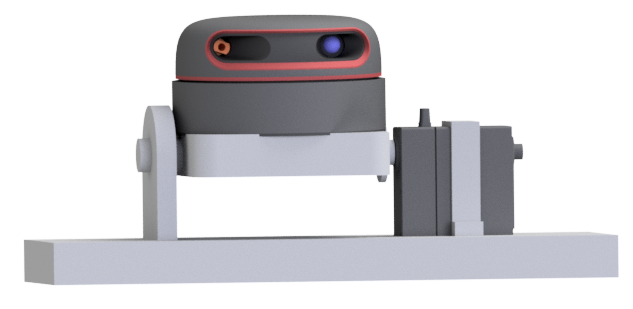
\includegraphics[width=.45\textwidth]{images/lidar_3d.png}}
%        \subfigure[]{\label{fig:lidar3Db}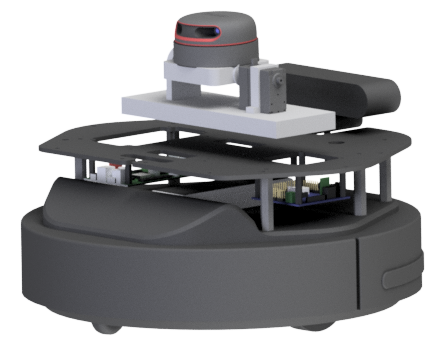
\includegraphics[width=.45\textwidth]{images/lidar_wKbki.png}}
%        \subfigure[]{\label{fig:lidar3Dc}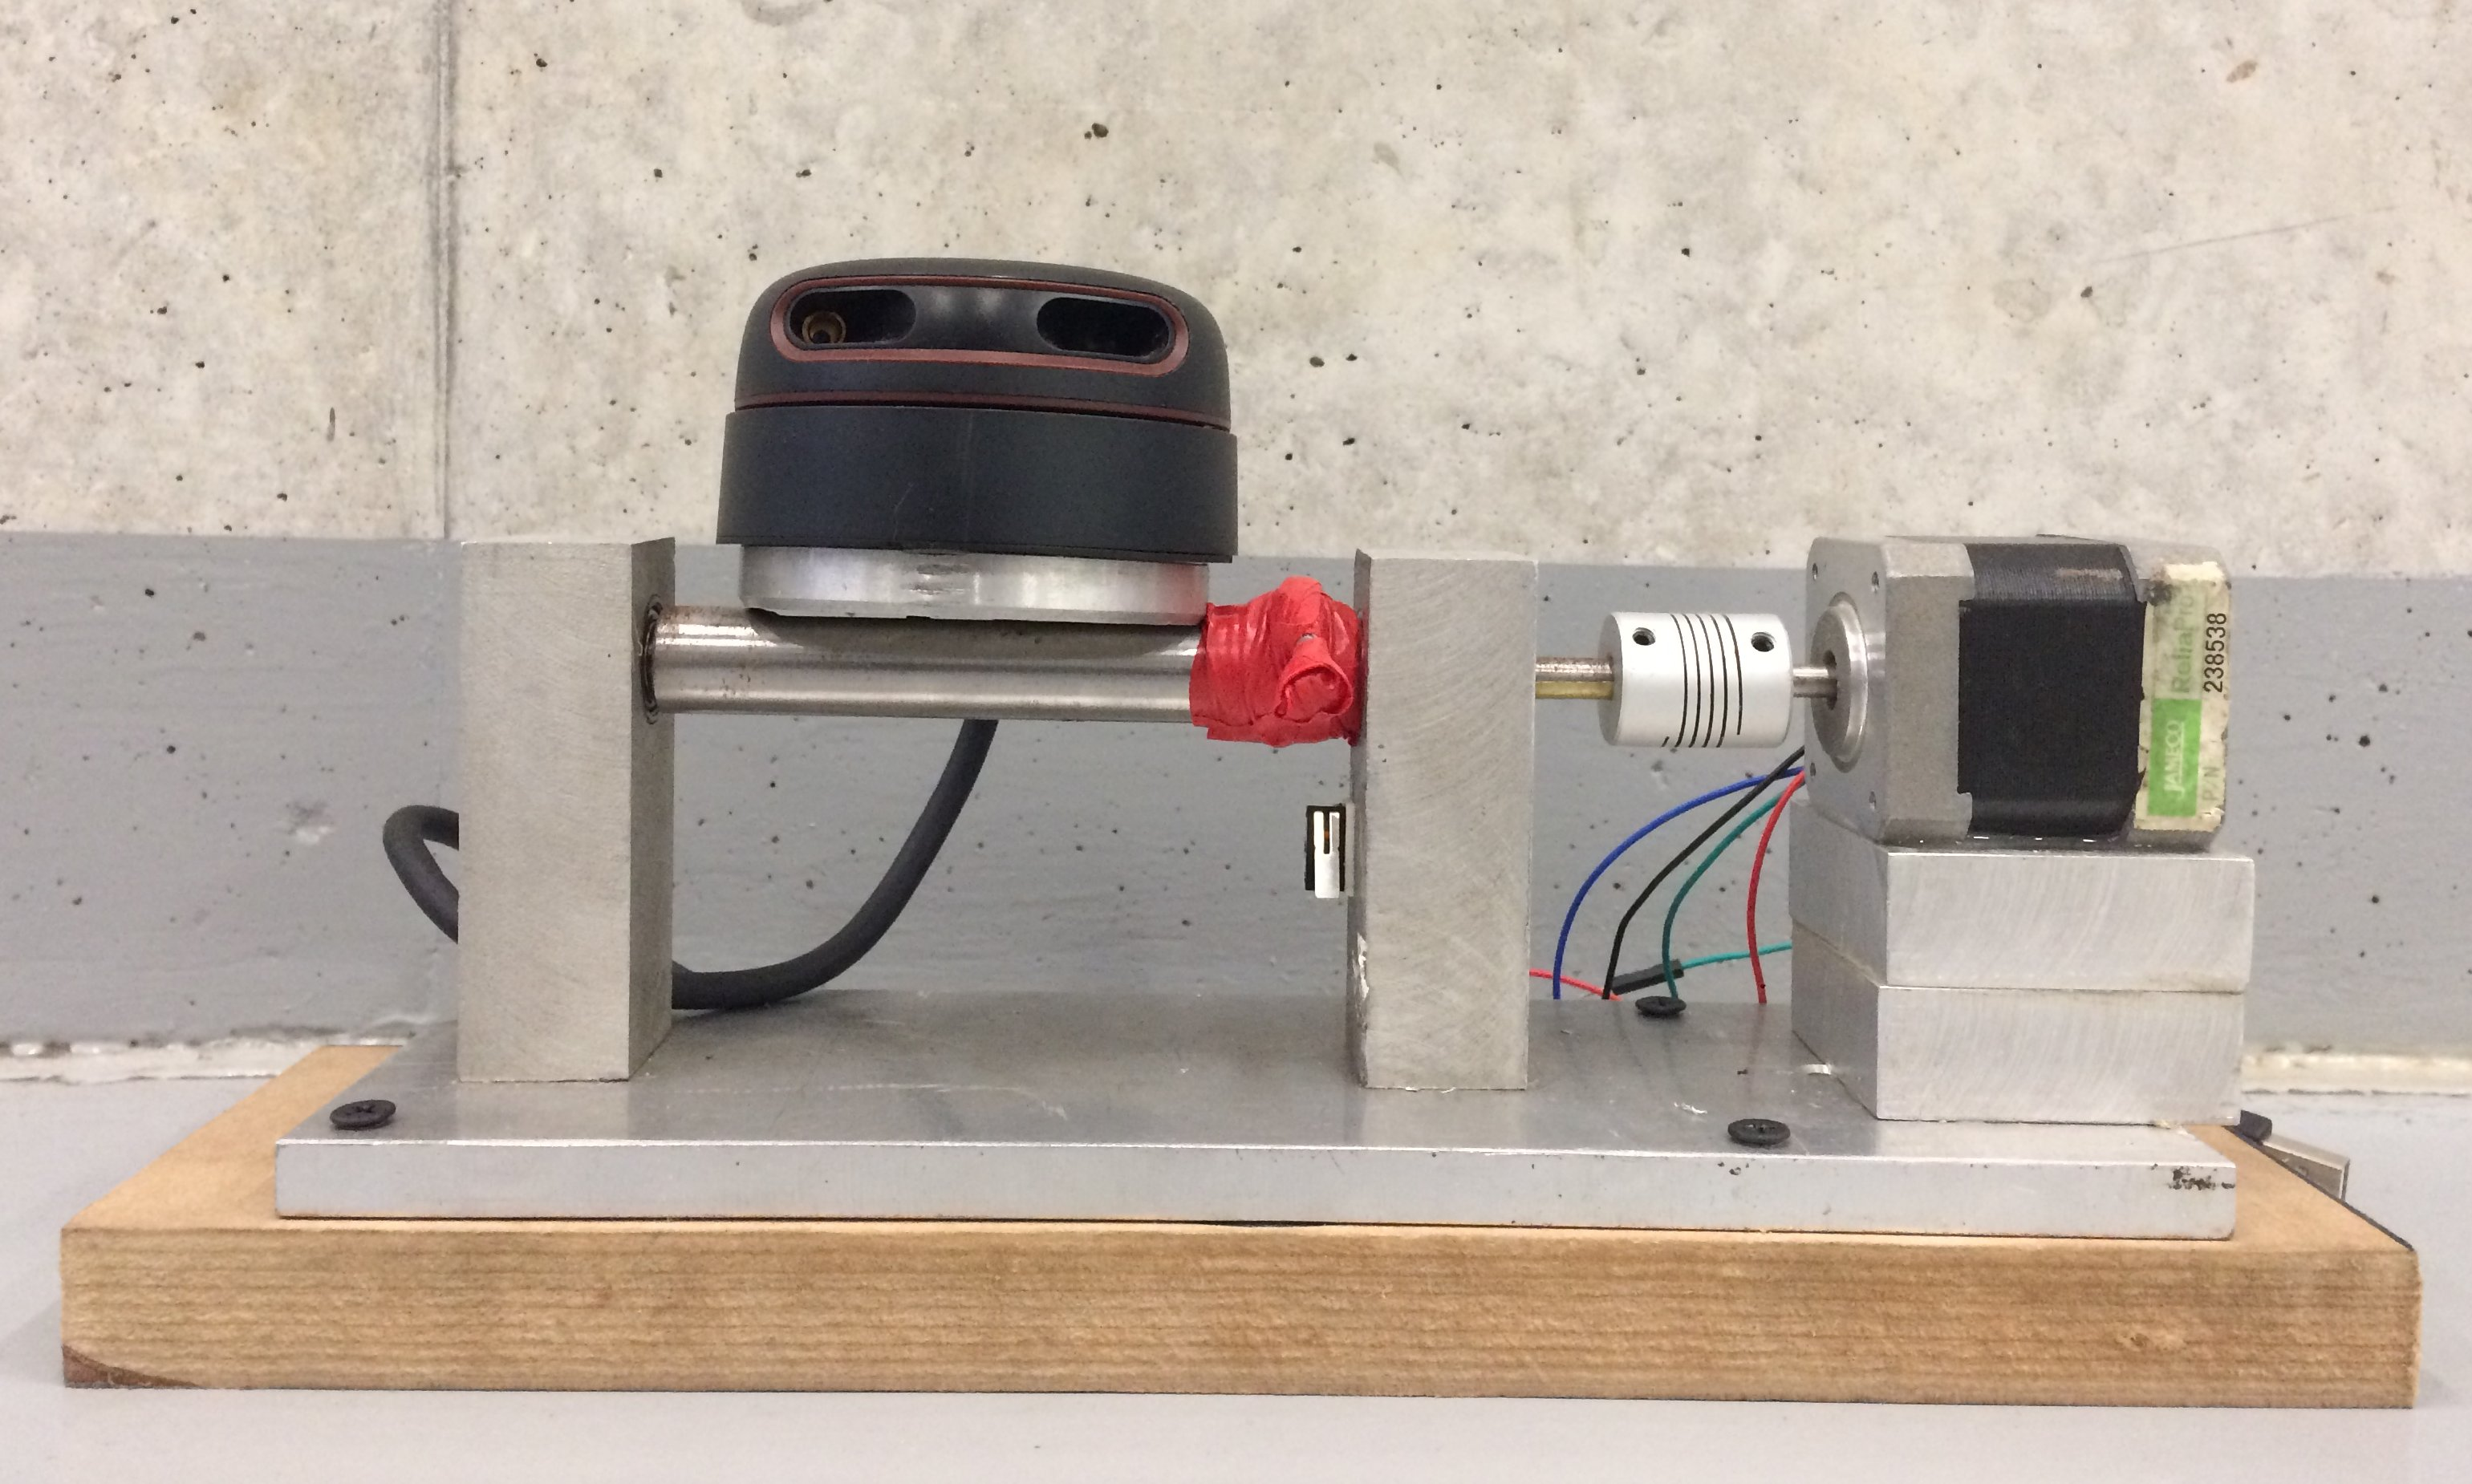
\includegraphics[width=.70\textwidth]{images/LIDAR_SIST.JPG}}
%    \end{center}
\begin{figure}%[ht!]
  \centering
  \begin{tabular}{cc}
     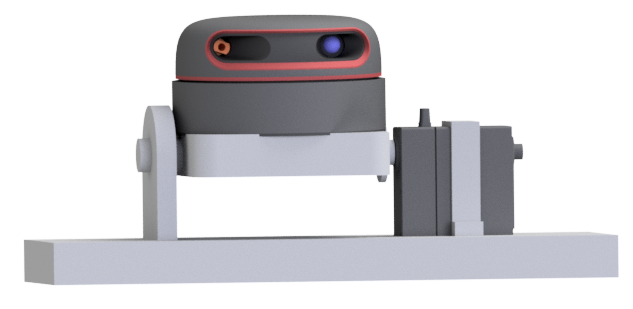
\includegraphics[width=0.45\linewidth]{images/lidar_3d.png}&
     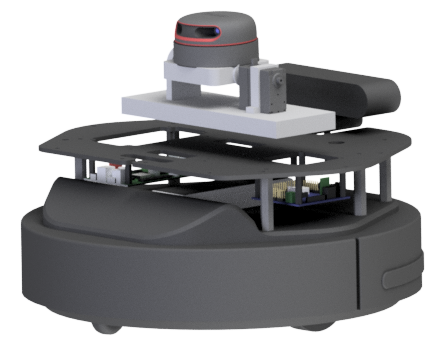
\includegraphics[width=0.45\linewidth]{images/lidar_wKbki.png}\\
    (a) & (b)\\
    \multicolumn{2}{c}{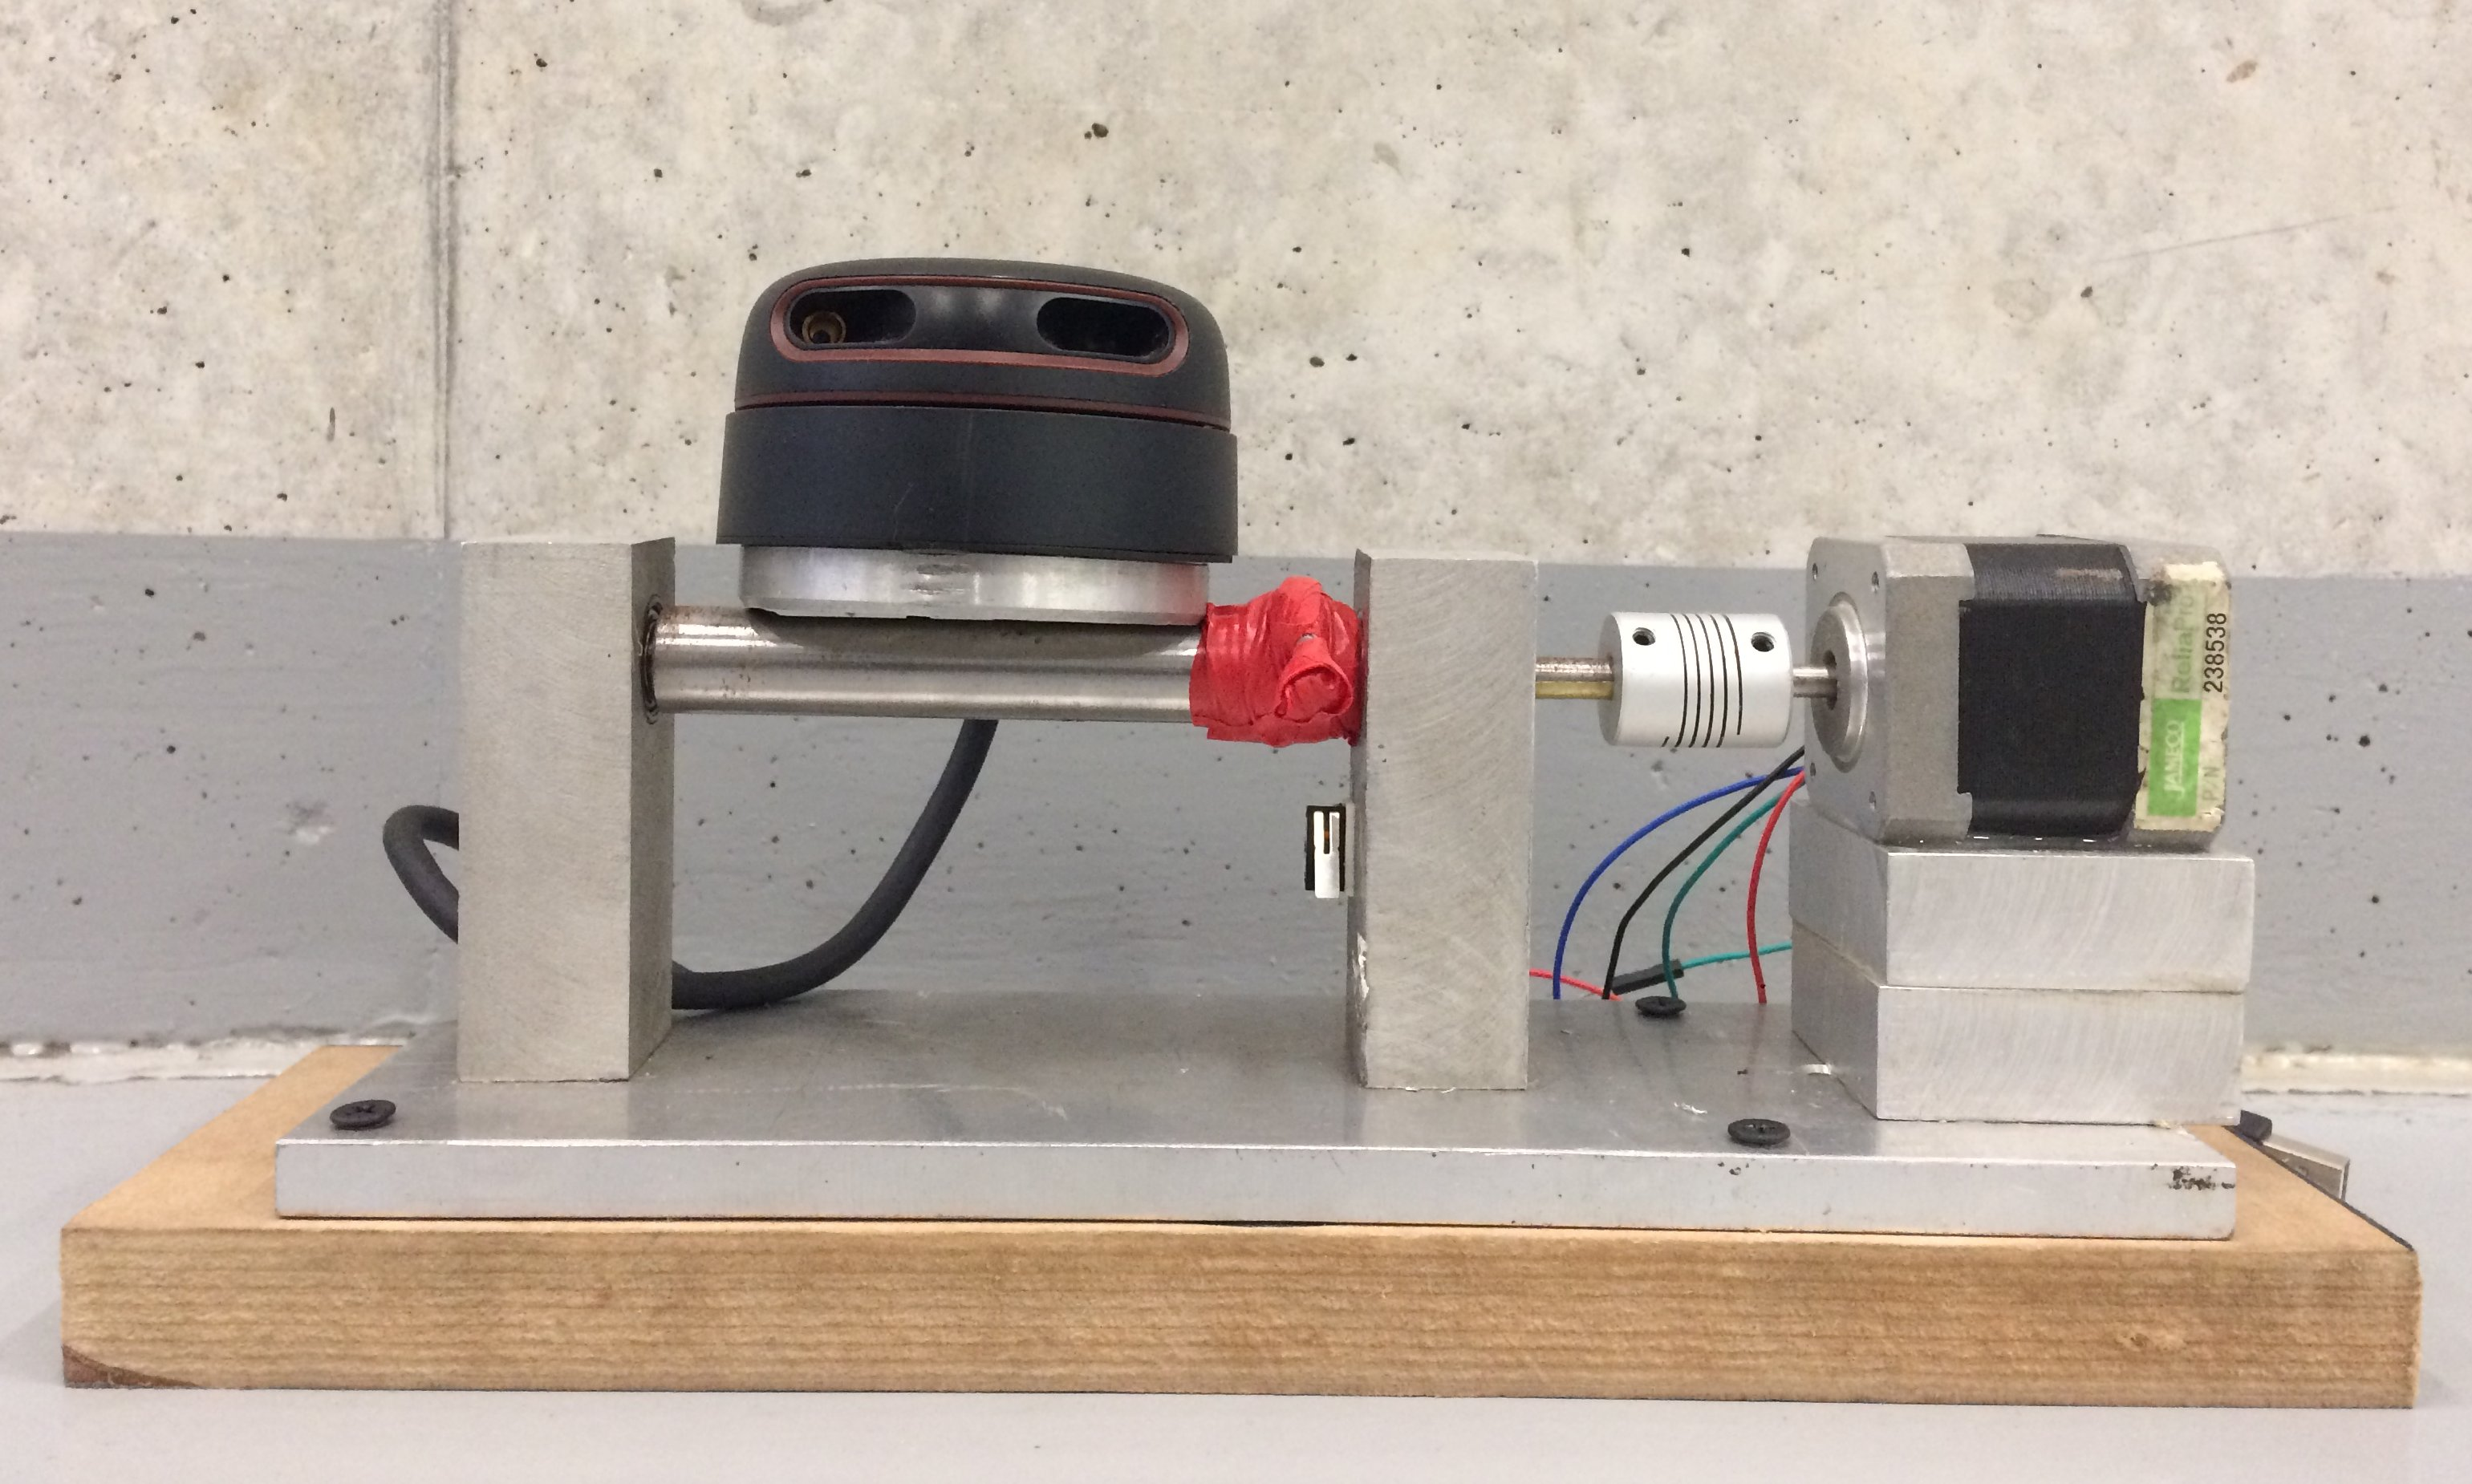
\includegraphics[width=0.70\linewidth]{images/LIDAR_SIST.JPG}}\\
    \multicolumn{2}{c}{(c)}
  \end{tabular}
  \captionsetup{font=footnotesize}
    \caption{\label{f:lidar3D}Diseño del sistema mecánico, desarrollado en un programa CAD. En (a) se 
    muestra el diseño en CAD del sistema mecánico, en (b) se muestra la forma en que va ser colocado 
    el sistema mecánico en el robot móvil kobuki y en (c) se muestra el diseño mecánico manufacturado 
    en aluminio, junto al sensor lidar y el motor paso a paso.}
\end{figure}
%\begin{figure}%[ht!]
%  	\centering \footnotesize
  %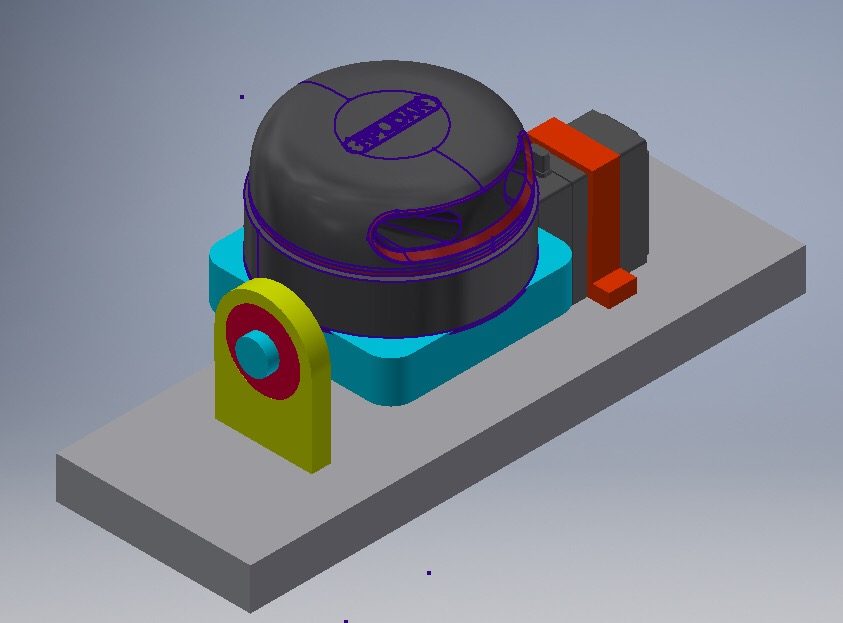
\includegraphics[width=0.40\textwidth]{images/lidar_3D.jpeg}
  %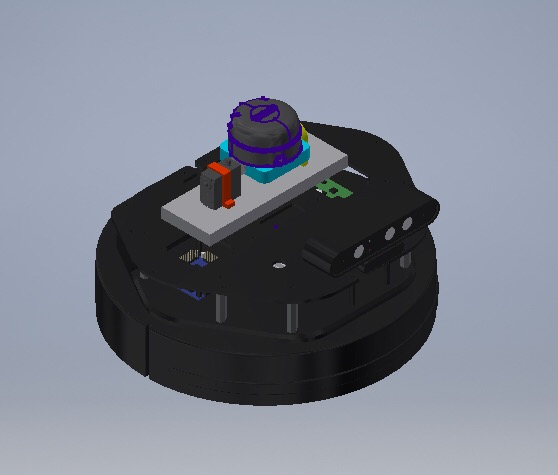
\includegraphics[width=0.35\textwidth]{images/kbki_lidar3D.jpeg}
%  	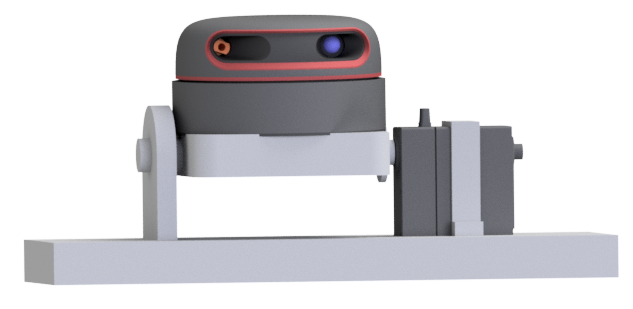
\includegraphics[width=0.40\textwidth]{images/lidar_3d.png}
%  	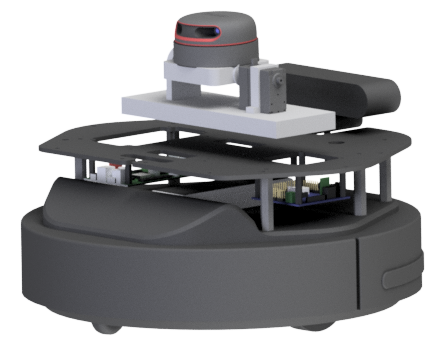
\includegraphics[width=0.40\textwidth]{images/lidar_wKbki.png}
%  	\\ $\qquad\qquad$ a. Sistema mecánico  $\qquad\qquad\qquad$  b. Sistema mecánico sobre el Kobuki
%  	\captionsetup{font=footnotesize}
%  	\caption{Sistema mec\'anico para el mapeo en tres dimensiones.}
%  	\label{f:lidar3D}
%\end{figure}

El sensor lidar es un sensor que permite construir mapas de dos dimensiones, como ya 
fue mencionado, este sensor realiza mediciones mientras va rotando en 360 \grad~. Para 
este trabajo de tesis se necesita desarrollar un sistema mecánico para que el robot 
pueda realizar mediciones en los tres ejes del plano cartesiano mientras se va 
desplazando. Por tal motivo, se realizó un diseño mecánico que es accionado por un motor
paso a paso. Este diseño está compuesto por una base que soporta al sensor lidar, asimismo, 
esta base tiene un eje en la parte inferior. Un extremo del eje de la base se encuentra 
acoplado al eje del motor paso a paso, mientras que el otro extremo se encuentra unida 
a un rodamiento que permite que la rotación del motor se realicé con el mínimo rozamiento. Este
sistema mecánico fue diseñado con el software mecánico \textit{Inventor}, como se muestra
en la Figura \ref{f:lidar3D}a.

El sistema mecánico final fue manufacturado, en aluminio, con las características mencionadas
anteriormente agregando un switch de autocalibración. Como se puede ver en la Figura 
\ref{f:lidar3D}c, el switch se encuentra en la parte inferior del eje de la base. La idea 
principal de este sistema de autocalibración es decirle al motor paso a paso en que posición 
debe considerar el ángulo 0\grad~. Una vez que este switch es accionado, el sensor lidar se 
coloca en la posición como se muestra en la Figura \ref{f:FrameSitemaMecanico}, a partir de esta 
posición el sistema mecánico hace que el sensor lidar rote hacia atrás y hacia adelante teniendo 
un ángulo de apertura desde $-88$\grad~ a $+88$\grad. El motor paso a paso tiene una resolución
de 1\grad~. La rotación del motor en el rango de $\pm$ 88\grad~ hace que el sensor lidar pueda 
tomar medidas en los tres ejes del plano cartesiano $(\mayusx,\mayusy,\mayusz)$.

%este va realizando mediciones mientras va rotando 360\grad~
%El sensor lidar permite construir mapas en dos dimensiones ya que este va midiendo 
%distancias mientras va rotando en 360\grad ~, pero para el alcance de este proyecto de 
%tesis se necesita que el robot pueda mapear el entorno en tres dimensiones. Para este
%objetivo se realizó un diseño mecánico, como se muestra en la Figura \ref{f:lidar3D}a. Este
%diseño permite que el sensor lidar pueda tener un ángulo de medición de $\pm$ 15\grad en el 
%eje $Z$. El sistema mecánico consiste en una base donde el sensor lidar se encuentra acoplada, 
%y a su vez este esta unido a un servomotor por medio de un eje. El servomotor esta programado para 
%que se mueva en un rango de $\pm$ 15\grad~ para que el sensor pueda tomar medidas 
%en el eje $Z$. 
\begin{figure}[ht!]
\centering \footnotesize
 %{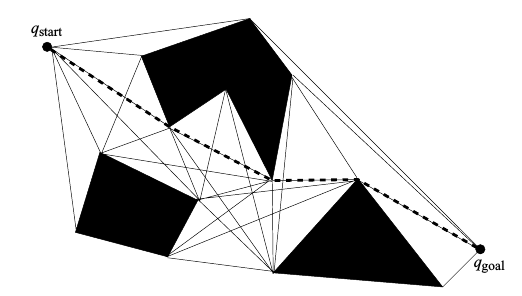
\includegraphics[width=0.60\linewidth]{images/shortPath_visibilityGraph.png}}
 {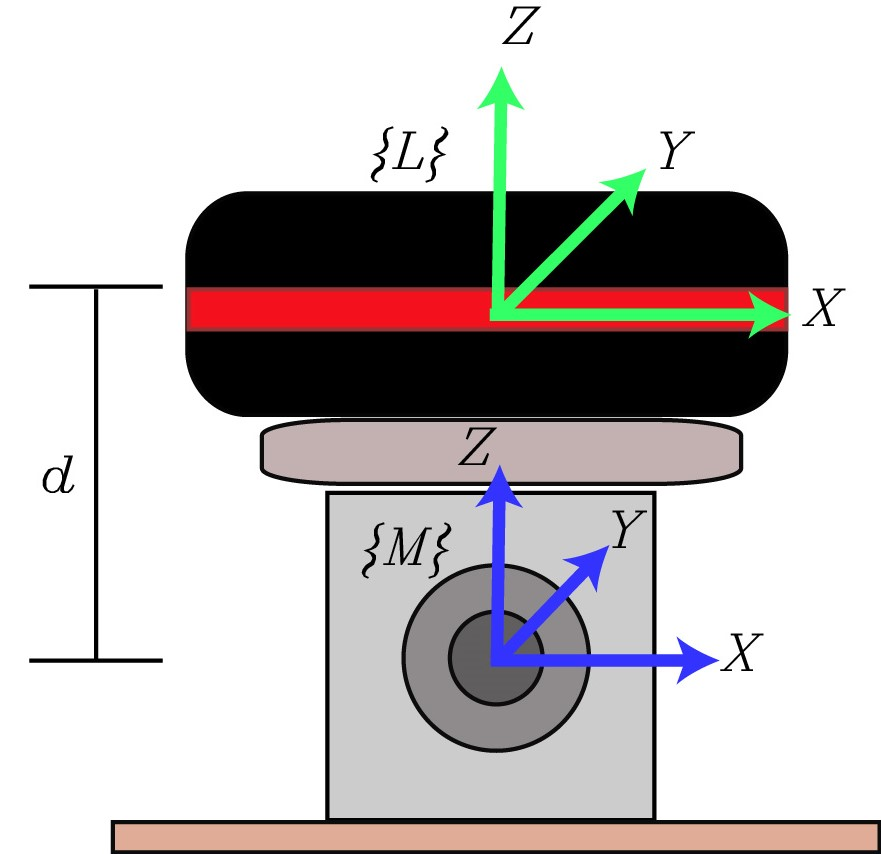
\includegraphics[width=0.55\linewidth]{images/lidar_kbki.jpg}}
 \captionsetup{font=footnotesize}
 \caption{Representación gráfica de los sistemas de referencia del sistema 
 mecánico. Donde $M$ y $L$ son los sistemas de referencia del motor paso a 
 paso y del sensor lidar.}
\label{f:FrameSitemaMecanico}
\end{figure}

\begin{figure}%[ht!]
     %\begin{center}
     \centering
     \begin{tabular}{cc}
        %\subfigure[]{\label{fig:etiquetaA}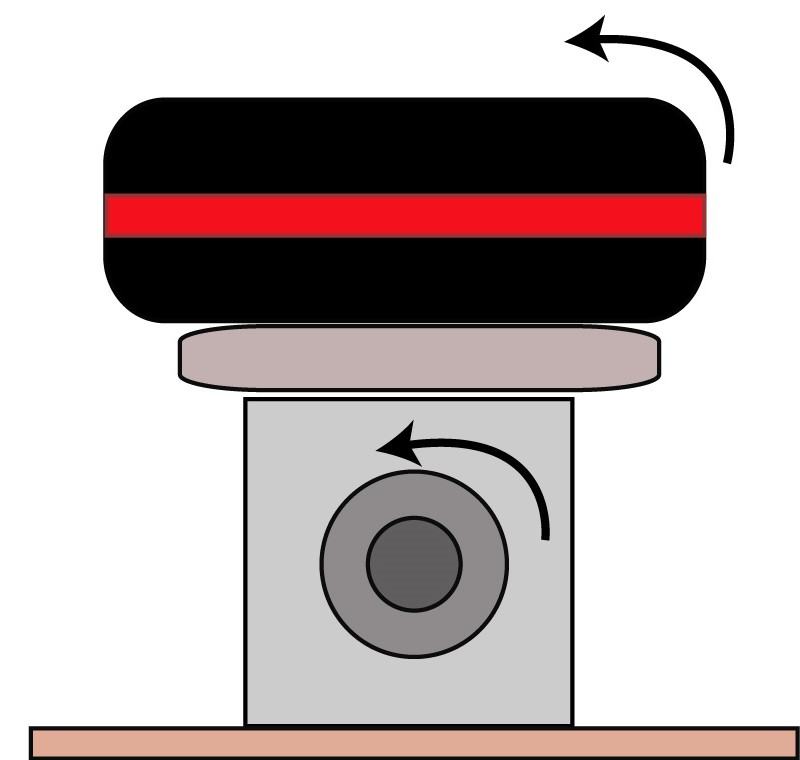
\includegraphics[width=.35\textwidth]{images/lidar_rot_tras2.jpg}}
        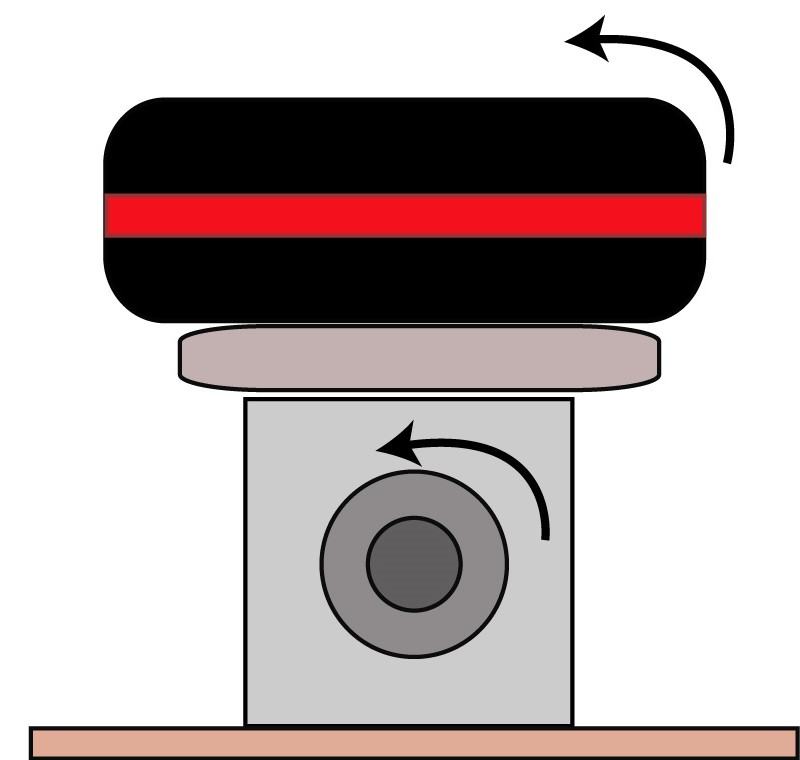
\includegraphics[width=.40\textwidth]{images/lidar_rot_tras2.jpg}&
        %\subfigure[]{\label{fig:etiquetaB}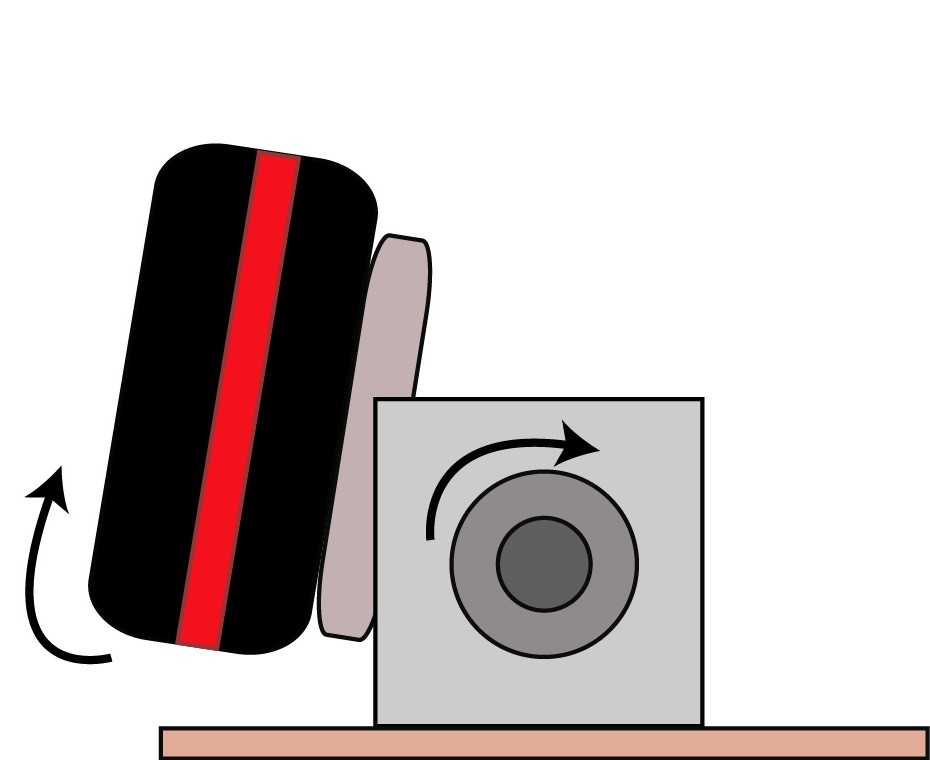
\includegraphics[width=.35\textwidth]{images/lidar_rot_tras3.jpg}}
        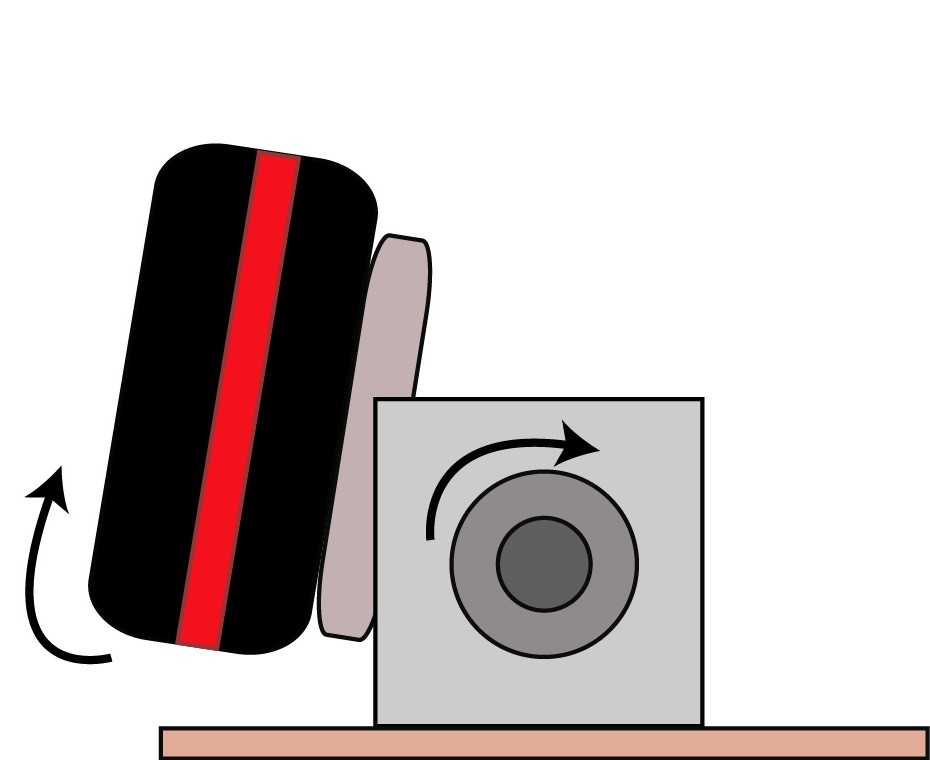
\includegraphics[width=.40\textwidth]{images/lidar_rot_tras3.jpg}\\
        (a)&(b)\\
        %\subfigure[]{\label{fig:etiquetaC}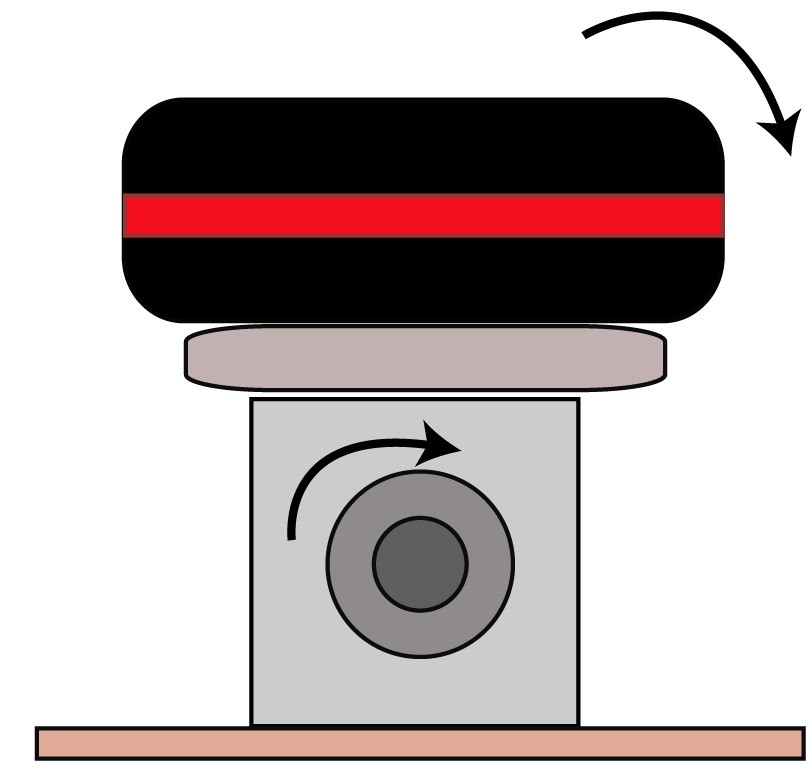
\includegraphics[width=.35\textwidth]{images/lidar_rot_tras.jpg}}
        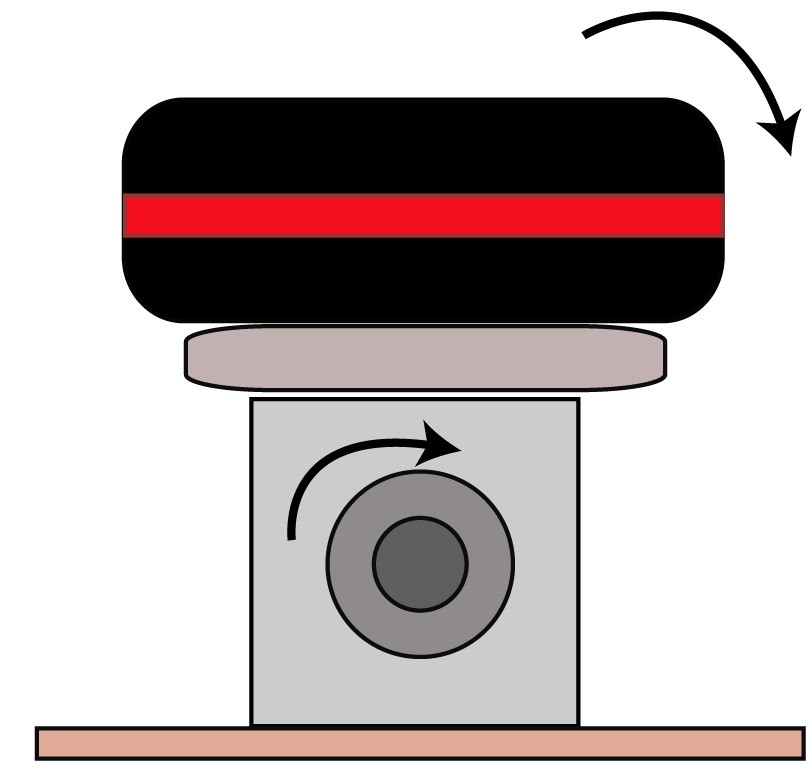
\includegraphics[width=.40\textwidth]{images/lidar_rot_tras.jpg}&
        %\subfigure[]{\label{fig:etiquetaD}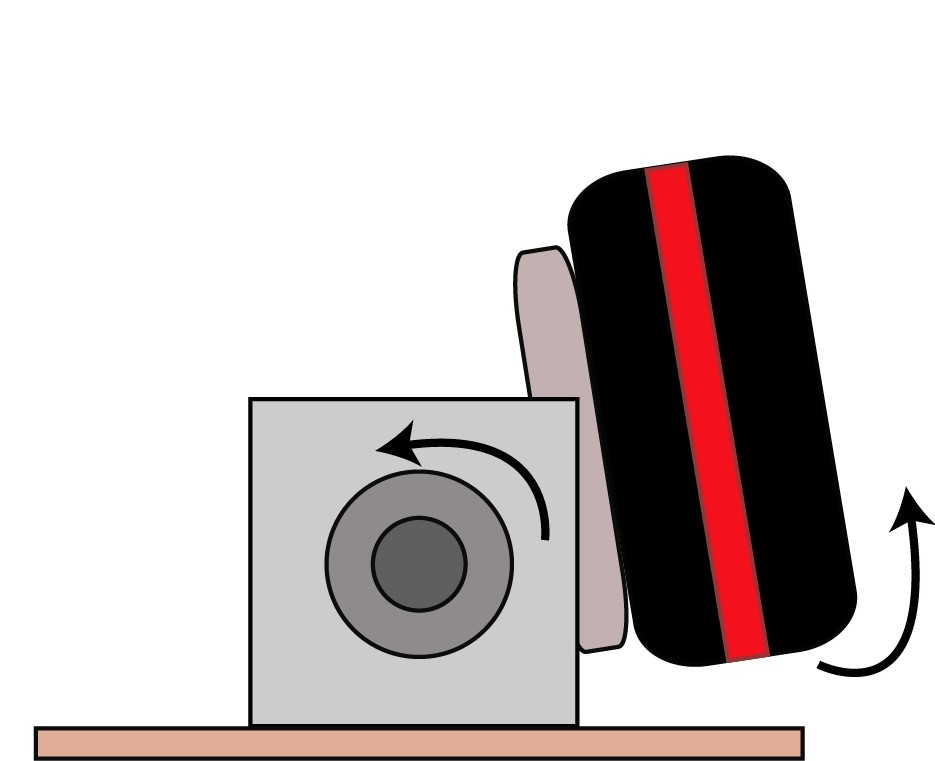
\includegraphics[width=.35\textwidth]{images/lidar_rot_tras1.jpg}}
        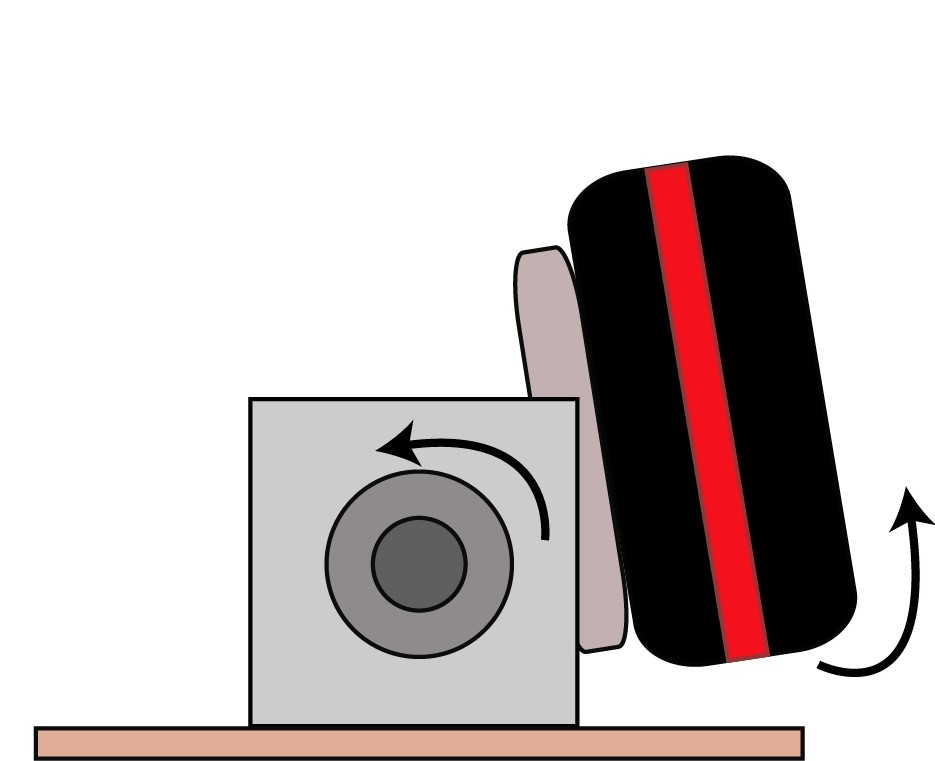
\includegraphics[width=.40\textwidth]{images/lidar_rot_tras1.jpg}\\
        (c)&(d)
    %\end{center}
    \end{tabular}
  \captionsetup{font=footnotesize}
    \caption{\label{f:Rot3D}Representación gráfica de los movimientos de rotación del sistema 
    mecánico.En (a) se muestra la posición inicial (0\grad) rotando hacia la izquierda, en (b) se 
    muestra el sensor lidar rotado hacia el ángulo $-88$\grad~ y rotando hacia la derecha. En (c) 
    se muestra que el sensor lidar regreso a su posición original (0\grad) y va rotar hacia la 
    derecha. En (d) se muestra el sensor lidar en el ángulo $88$\grad~ rotando hacia la izquierda.}
\end{figure}

Para generar el mapa en tres dimensiones se debe tener en consideración los sistemas de referencia 
de todos los componentes del sistema mecánico, en este caso el sensor lidar y el motor paso a paso
como se muestra en la Figura \ref{f:FrameSitemaMecanico}. Este sistema genera un movimiento de rotación
y traslación que son considerados dentro de las ecuaciones matemáticas para obtener los valores en los 
tres ejes del plano cartesiano. Una vez que el sistema mecánico es autocalibrado accionado por el 
switch, el sensor lidar es posicionado como muestra la Figura \ref{f:Rot3D}a, en esa posición se 
considera que el ángulo del motor paso a paso es 0\grad. Luego el sensor lidar se comienza a rotar 
hacia el lado derecho hasta que llega al ángulo $-88$\grad~ (ver Figura \ref{f:Rot3D}b). Una vez que
el motor paso a paso llega al ángulo $-88$\grad este comienza a girar hacia la izquierda hasta 
que llega al ángulo $88$\grad, como se muestran en las Figuras \ref{f:Rot3D}c y \ref{f:Rot3D}d. El 
ángulo de apertura que tiene el motor paso a paso hace que el sensor lidar pueda tener un 
panorama más amplio para poder tomar mediciones dentro de un ambiente.

El mapa tridimensional se construye con las mediciones del sensor lidar y los ángulos del motor paso
a paso. Para esto primero se convierte los datos del sensor lidar, es decir hacer una conversión 
de coordenadas polares a coordenadas cartesianas. Las ecuaciones utilizadas son:
\begin{align*}
	x &= rcos(\theta_{L}), \\
	y &= rsen(\theta_{L}),
\end{align*}
donde $r$ es la distancia medida por el sensor y $\theta_{L}$ es el ángulo de rotación del sensor 
lidar por cada medición que realiza.

Los valores del sensor lidar convertidos debe ser llevado al sistema de referencia del motor paso a 
paso, para esto se utiliza una matriz homogénea que contiene los componentes de rotación y traslación
de todo el sistema mecánico. La matriz de transformación homogénea es representada como:
\begin{align*}
	T_{L}^{M} &= R_{y}(\phi_{M}) T_{z}(d), \\
\end{align*}
%\begin{align}
%	\tilde{p}^{M} = T_{L}^{M} \tilde{p}^{L}
%	\label{eqn:MatrizHomogenea}
%\end{align}
donde $\phi_{M}$ representa al ángulo de rotación del motor paso a paso y $d$ a la distancia entre el 
sistema de referencia del sensor lidar y el sistema de referencia del motor paso a paso, como se 
puede ver en la Figura \ref{f:FrameSitemaMecanico}. La matriz  de transformación homogénea
tiene una matriz de rotación, denotado por $R_{y}(\phi_{M})$, originado por la acción del 
motor paso a paso en el eje $\mayusy$ y una matriz de traslación, denotado por $T_{Z}(d)$, en el 
eje $\mayusz$ originado la pequeña distancia que existe entre los sistemas de referencia 
del sistema mecánico. La posición y orientación de los valores en los tres ejes del plano
cartesiano (nube de puntos) es representada como:
\begin{align}
	\tilde{p}^{L} = T_{L}^{M} \tilde{p}^{M}
	\label{eqn:MatrizHomogenea}
\end{align}
donde $\tilde{p}^{L}$ representa la coordenada homogénea con respecto al sistema de referencia del sensor
lidar, $T_{L}^{M}$ es la matriz homogénea descrita anteriormente y $\tilde{p}^{M}$ es la coordenada 
homogénea con respecto al sistema de referencia del motor paso a paso. La multiplicación de estas matrices
ayuda a encontrar las coordenadas en los ejes ($\mayusx,\mayusy,\mayusz$) del ambiente
que se esta mapeando.

\subsection{Prototipo Final}
\begin{figure}%[ht!]
	\centering \footnotesize
	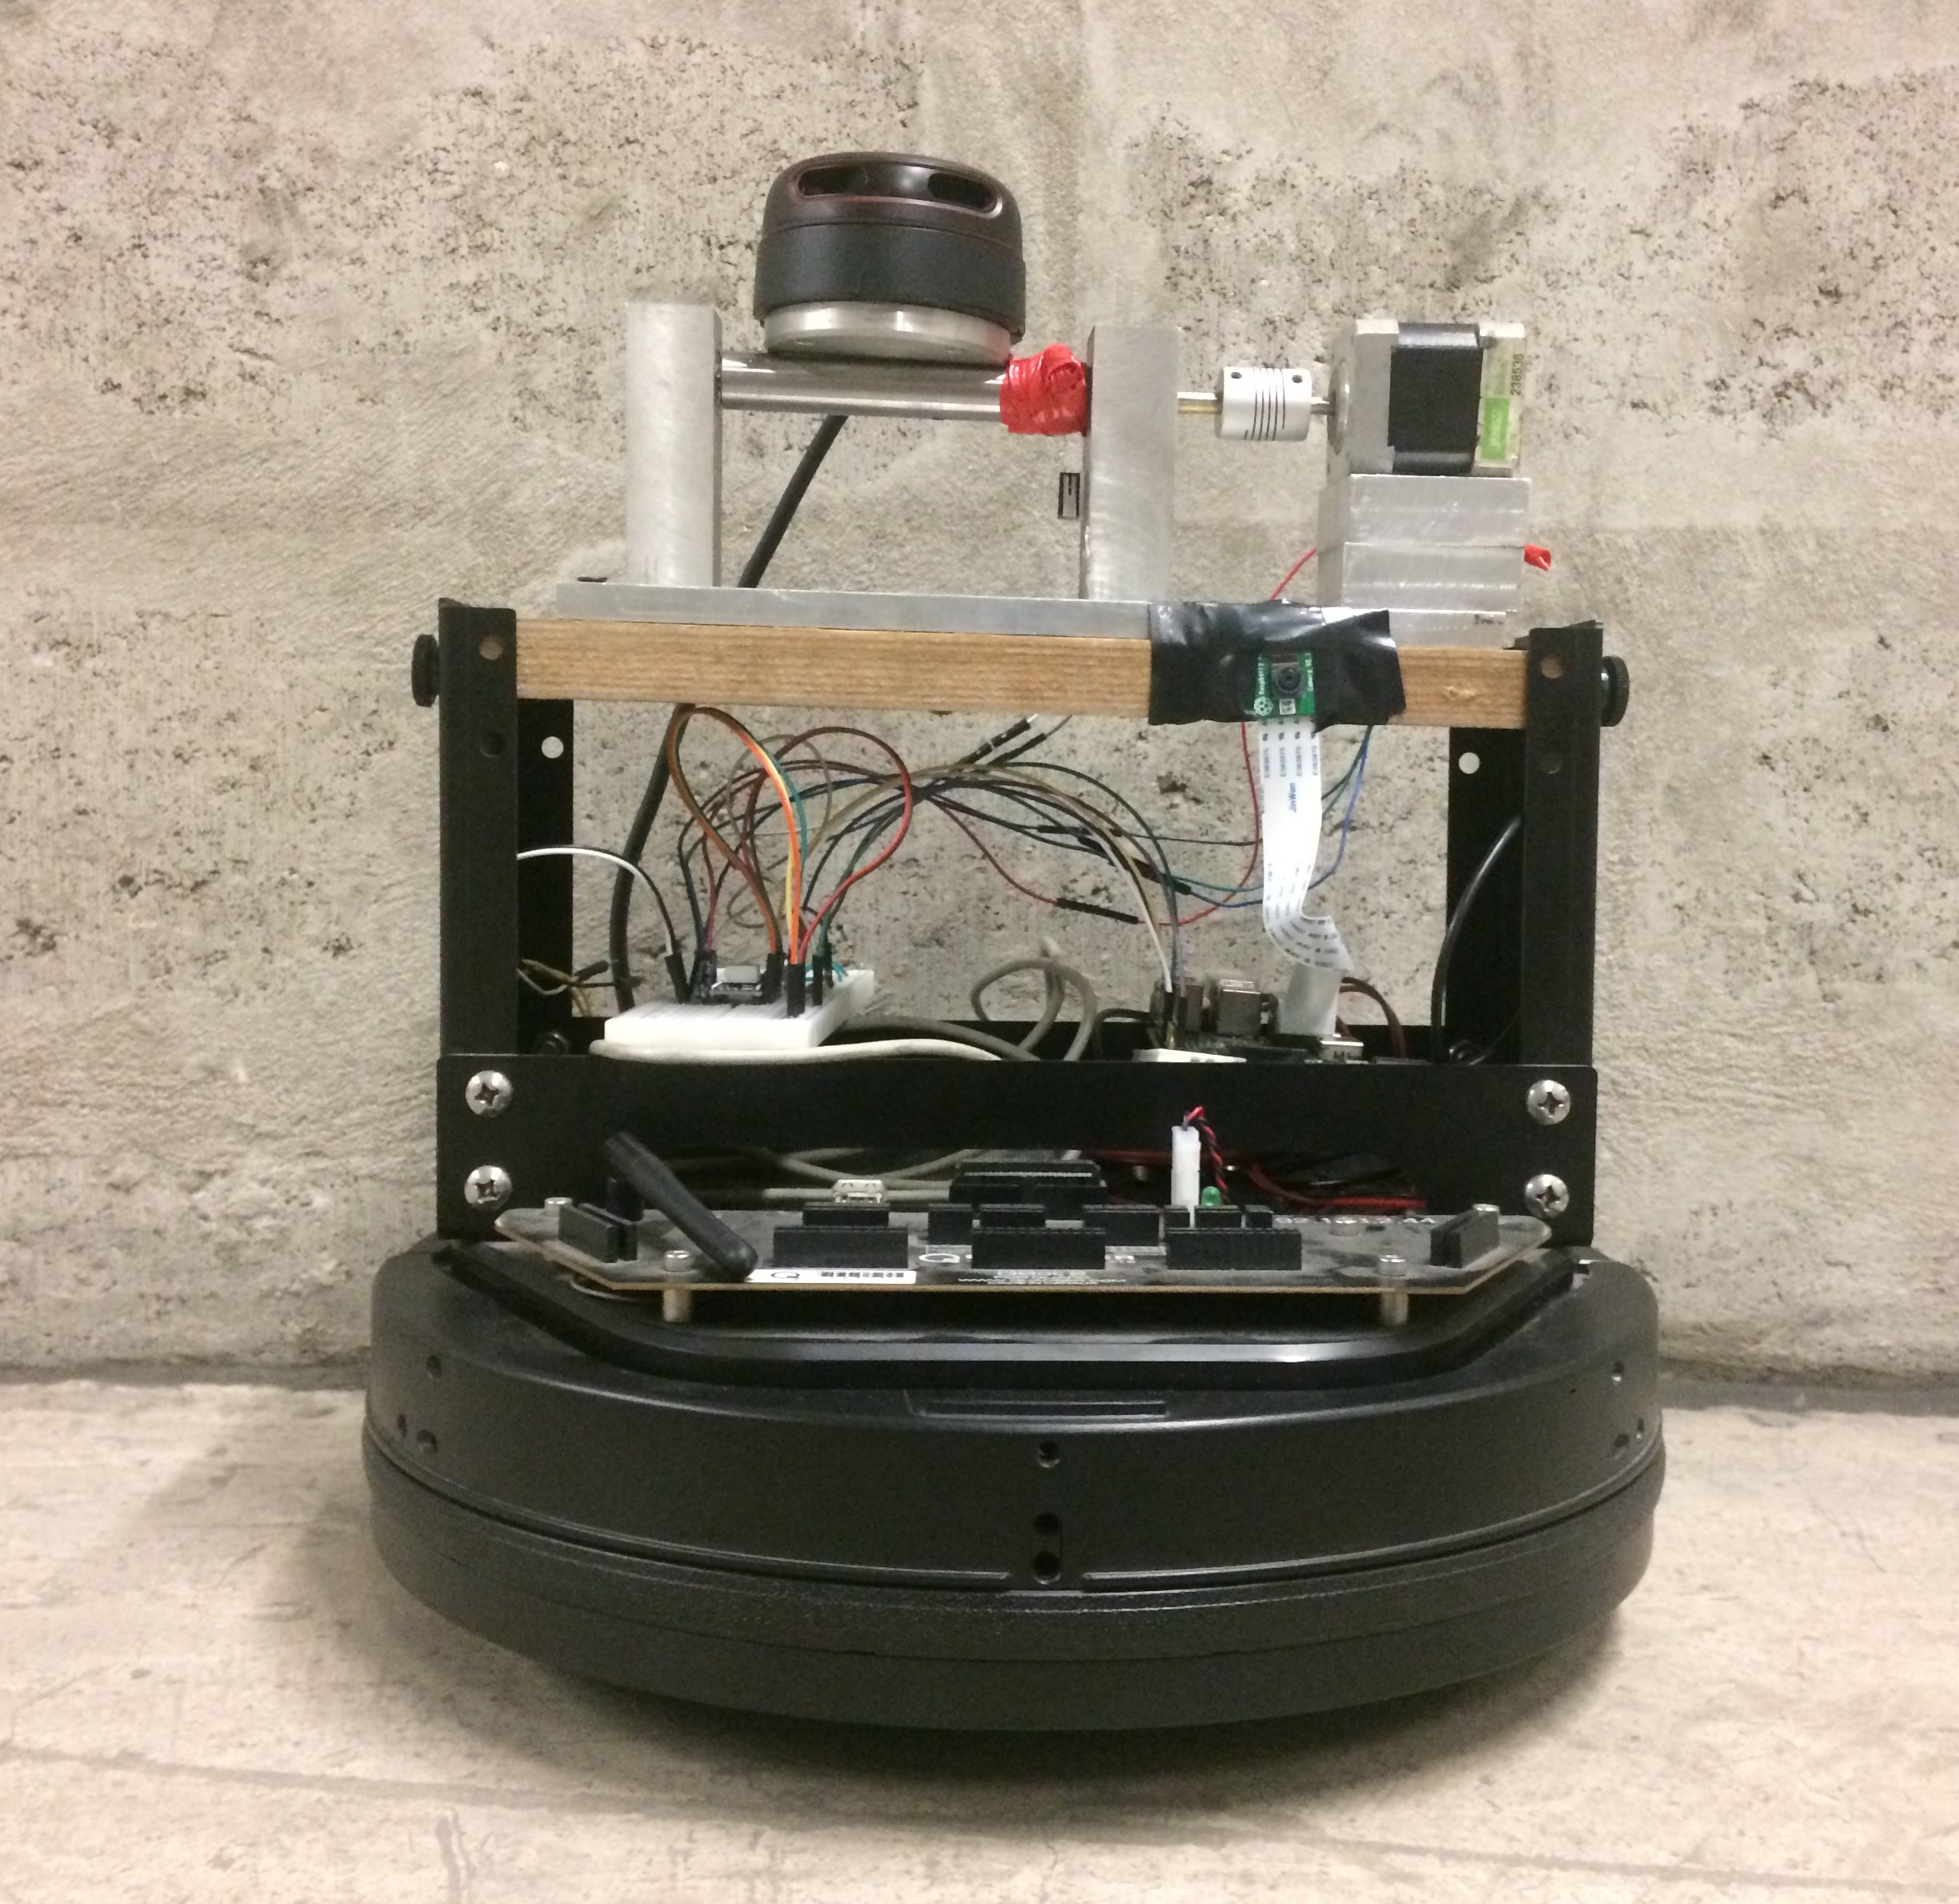
\includegraphics[width=0.65\textwidth]{images/ProtFinal.JPG}
	\captionsetup{font=footnotesize}
	\caption{Esta figura muestra el prototipo final que fue utilizado para realizar las pruebas
	de navegación autónoma y mapeo de un ambiente en tres dimensiones. }
	\label{fig:ProtoFinal}
\end{figure}
El prototipo final del presente trabajo de tesis se muestra en la Figura \ref{fig:ProtoFinal}, 
este robot puede desplazarse de forma autónoma en un ambiente desconocido y a su vez 
puede generar un mapa en tres dimensiones del lugar. El prototipo está compuesto por un robot
móvil diferencial Kobuki, un sensor lidar y un motor paso a paso, estos se encuentran conectados
a un microcontrolador Raspberry Pi 3. Este microcontrolador es usado para poder controlar 
todos los componentes mencionados y poder almacenar la información de la nube de puntos que genera 
el sistema mecánico.

%\section{Movimiento del Robot y Mapeo}

%\subsection{Control de Bajo Nivel}

\section{Generación de Trayectoria basado en Campos Potenciales}
\label{sec:autonomia}

%\begin{figure}[ht!]
%     \begin{center}
%        \subfigure[]{\label{fig:etiquetaB}\includegraphics[width=.49\textwidth]{images/attr_force.png}}%NO CAMBIAR
%        \subfigure[]{\label{fig:etiquetaC}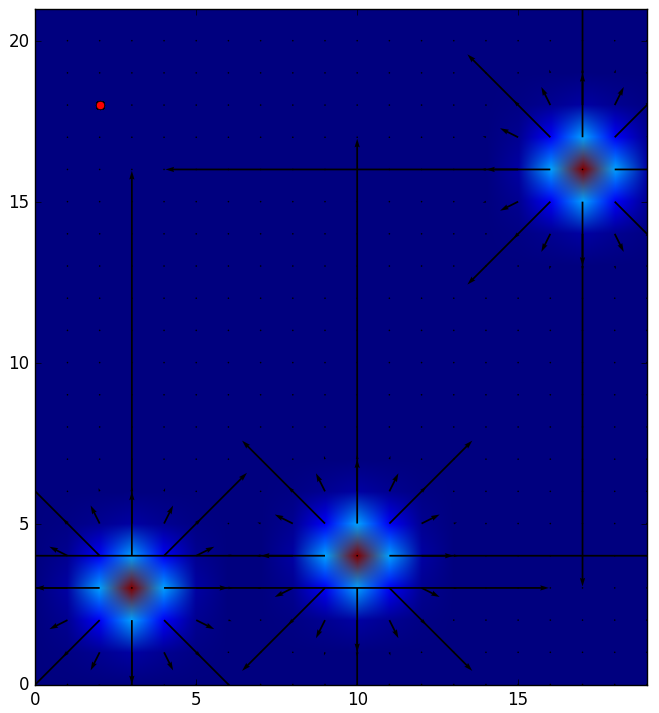
\includegraphics[width=.49\textwidth]{images/rep_force.png}}
%        \subfigure[]{\label{fig:etiquetaC}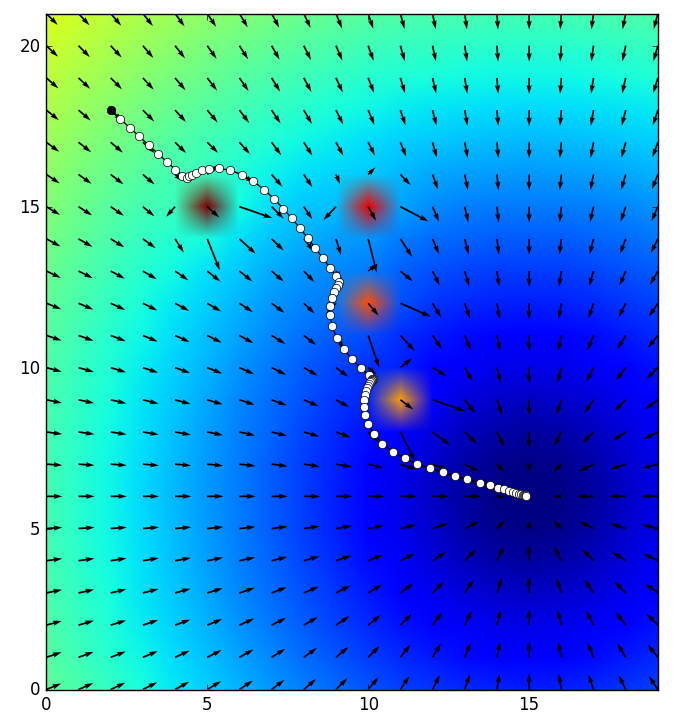
\includegraphics[width=.49\textwidth]{images/nav_force.png}}
%    \end{center}
\begin{figure}%[ht!]
  \centering
  \begin{tabular}{cc}
     \includegraphics[width=0.45\linewidth]{images/attr_force.png}&
     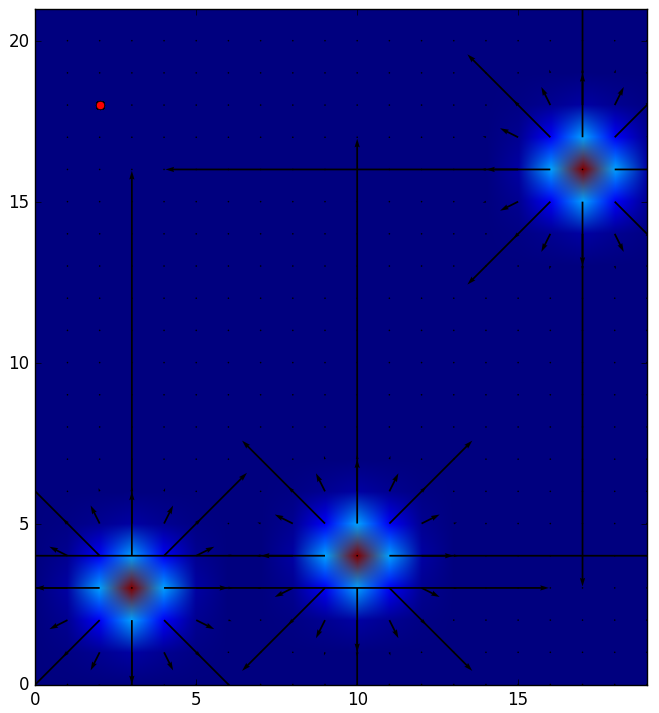
\includegraphics[width=0.45\linewidth]{images/rep_force.png}\\
    (a) & (b)\\
    \multicolumn{2}{c}{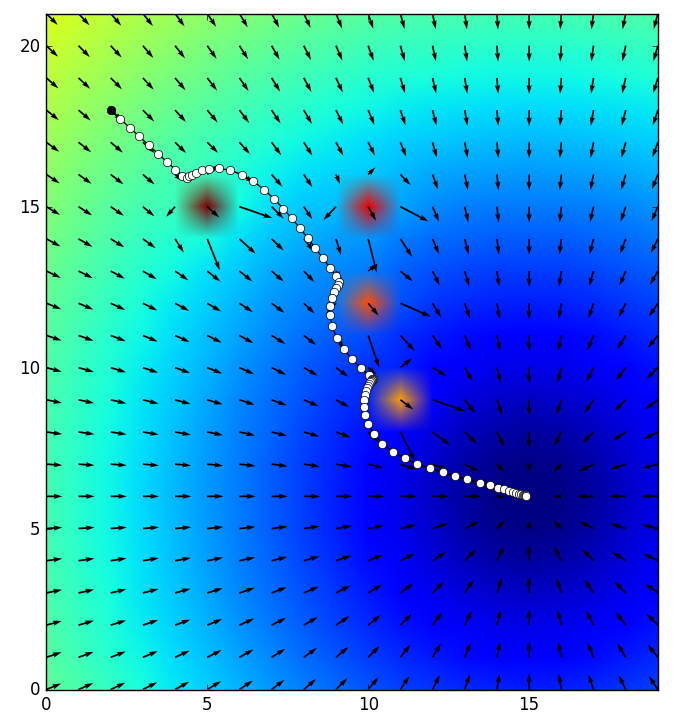
\includegraphics[width=0.50\linewidth]{images/nav_force.png}}\\
    \multicolumn{2}{c}{(c)}
  \end{tabular}
  \captionsetup{font=footnotesize}
    \caption{\label{f:APF}En esta figura se muestra las pruebas para el algoritmo de campo potencial 
    artificial. En (a) se muestra la prueba para las fuerzas de atracción, en (b) se muestra la
    prueba de las fuerzas de repulsión de cada uno de los obstáculos y en (c) se muestra la fuerza
    de navegación.}
\end{figure}
%\begin{figure}%[ht!]
%  	\centering \footnotesize
  %\subfloat[Attractive Force]{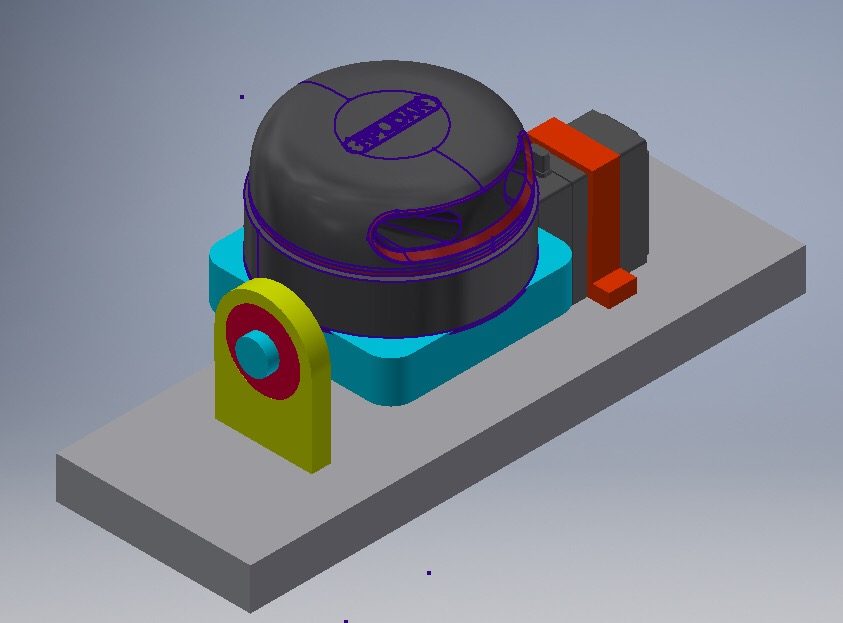
\includegraphics[width=0.16\textwidth]{images/lidar_3D.jpeg}}
  %~\subfloat[Repulsive Force]{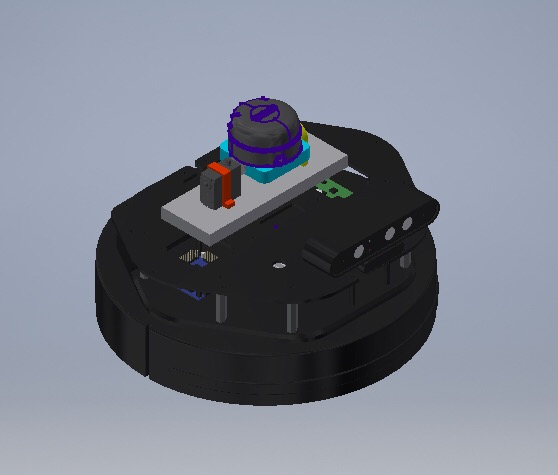
\includegraphics[width=0.16\textwidth]{images/kbki_lidar3D.jpeg}} 
%  	\includegraphics[width=0.40\textwidth]{images/attr_force.png}
%  	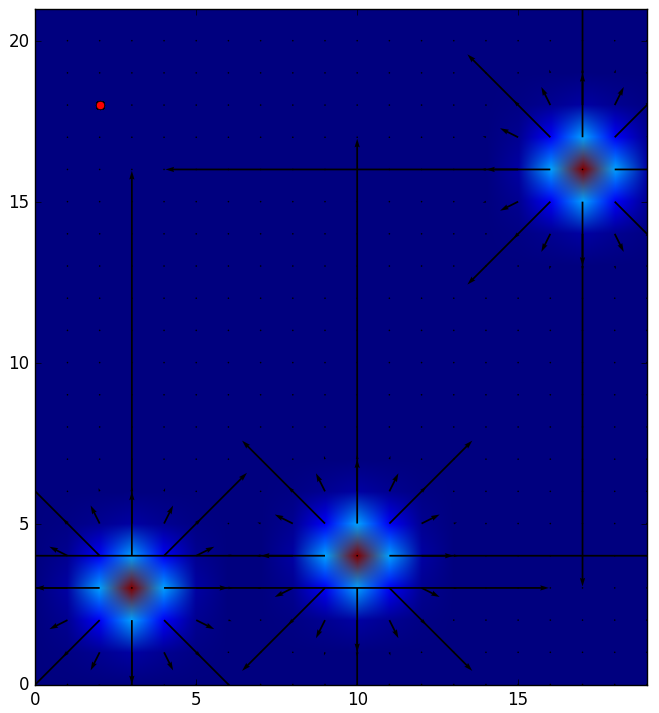
\includegraphics[width=0.40\textwidth]{images/rep_force.png}
%  	\\ $\qquad$ a. Fuerzas de atracción  $\qquad\qquad\qquad$  b. Fuerzas de repulsión
%  	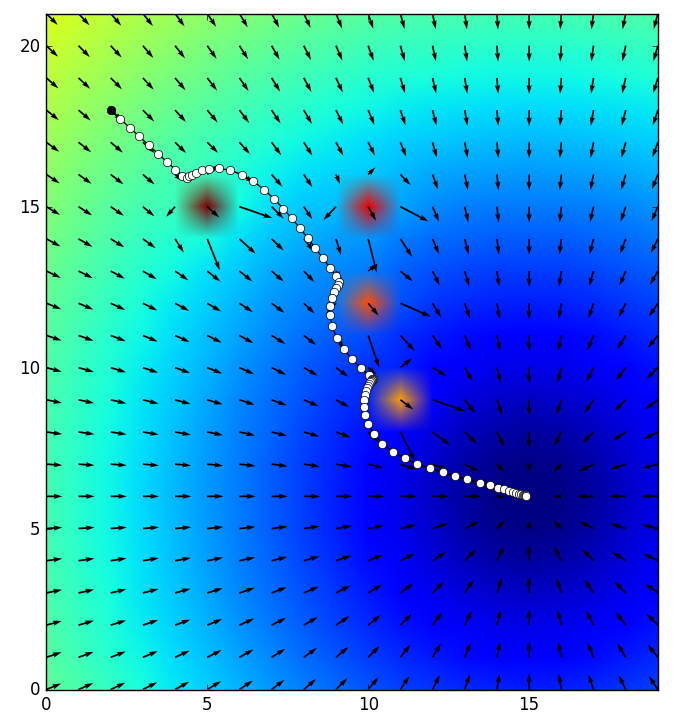
\includegraphics[width=0.45\textwidth]{images/nav_force.png}
%  	\\ $\qquad$ c. Fuerzas de navegación
  %\subfloat[Navigation Force]{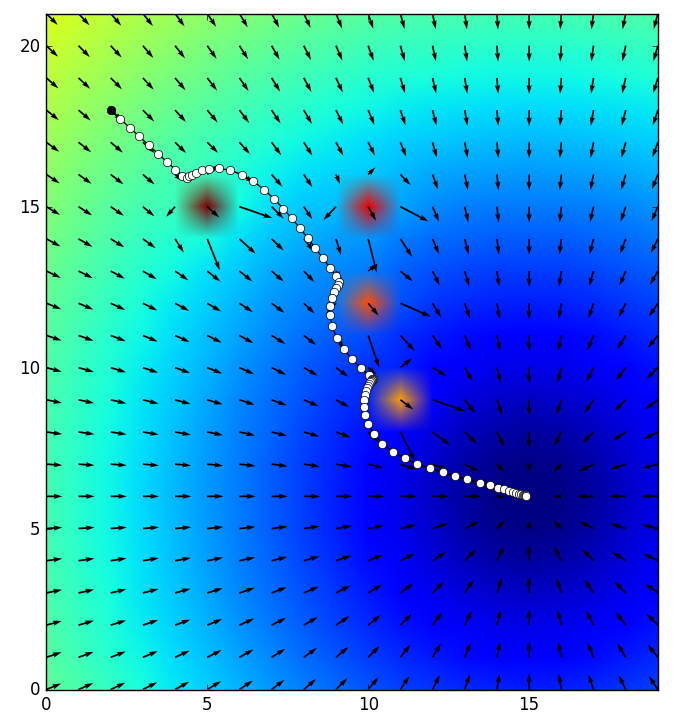
\includegraphics[width=0.16\textwidth]{images/nav_force.png}}
  % \subfloat[Attractive Force]{\includegraphics[width = 150mm]{attr_force.png}}
%  	\captionsetup{font=footnotesize}
%  	\caption{Pruebas para el algoritmo de campo potencial artificial.}
  %\label{f:lidar3D}
%  	\label{f:APF}
%\end{figure}
Para hacer que el robot se mueva a su objetivo final sin toparse con obstáculos, se 
hace uso de la teoría explicada en la sección \ref{sec:Campos Potenciales}. Primero, un 
objetivo final deseado $q_{g} =(x_{g}, y_{g}, \theta_{g})$ que describe la posición y la 
orientación se específica en términos del marco inercial. Entonces, los datos locales 
actuales del entorno se obtienen por medio de un sensor como un lidar, que fue usado en 
los experimentos, pero se puede usar cualquier otro sensor de profundidad. Estos datos 
proporcionan las posiciones de los obstáculos que se encuentran en el campo de visión del 
robot, y se utilizan como posiciones de obstáculos que definen el campo de repulsión. 

Usando el campo potencial definido por la posición deseada y los datos detectados, se toma un 
paso en la posición actual. Este paso da un pequeño incremento en la dirección y define la 
posición deseada que debe seguir el controlador polar. A medida que el robot se mueve, esta 
posición deseada también cambia según el campo potencial, guiando el movimiento hacia la meta 
y evitando los obstáculos. A medida que el robot se mueve, continúa escaneando y actualizando 
su mapa de obstáculos y, por lo tanto, actualizando todo el campo potencial compuesto por las 
partes atractivas y repulsivas.

Las fuerzas proporcionadas por el campo de potencial artificial se descomponen en 
magnitud y dirección que conducen continuamente al robot. Para mostrar cómo funciona el 
enfoque, se realiza una prueba en la computadora, que utiliza obstáculos 
colocados artificialmente y una posición deseada. La Figura \ref{f:APF}a muestra el campo 
de atracción y las fuerzas que guían hacia la posición deseada. El robot simulado se 
encuentra inicialmente en la esquina superior izquierda $q_{0} = (2,18)$ y se mueve hacia 
la meta $q_{goal} = (10,4)$ guiado por el campo. Los puntos blancos muestran la ruta que debe 
seguir el robot y que luego guiará al controlador. Un campo repulsivo puro se muestra en 
la Figura \ref{f:APF}b, donde se agregaron tres obstáculos en diferentes posiciones del espacio de 
trabajo. Cada obstáculo se proyecta como un círculo rojo debido a su gran magnitud dentro de 
su campo potencial, donde las fuerzas apuntan hacia afuera en cada obstáculo. La fuerza de 
navegación total compuesta por la superposición de las fuerzas de atracción y repulsión se 
muestra en la Figura \ref{f:APF}c.

\section{SLAM basado en Filtros de Part\'iculas}
\label{sec:GMAPPING}
Los filtros de partículas es un método que fue introducido en años recientes como un medio 
eficaz para resolver el problema de la localización y mapeo simultáneo 
\cite{nummiaro2003adaptive}. Para este trabajo de tesis se utilizo un paquete de código 
abierto llamado \textit{gmapping}, este paquete de \textit{ROS} (\textit{Robot Operating System}) 
emplea el algoritmo SLAM basado en filtros de partículas \cite{grisetti2007improved}, la teoría
de este algoritmo fue explicada en la sección \ref{sec:SLAM_FP}.

El SLAM basado en filtros de partículas consiste en que cada partícula lleva la información de 
un mapa del entorno. El cual se enfoca en calcular la probabilidad del mapa no solo utilizando 
la odometría del robot, sino también incluye las mediciones que hace un sensor, en este caso un 
sensor lidar que se encuentra encima del robot. Estas informaciones enviadas al algoritmo hace 
que la incertidumbre sobre la posición y orientación del robot disminuya. 

Uno de los principales problemas de la técnica SLAM basado en filtros de partículas es la cantidad 
de partículas requeridas para construir un mapa preciso. Este efecto es conocido como el 
problema del agotamiento de partículas. Por tal motivo el paquete \textit{gmapping} propone 
dos pasos para solucionar este problema. El primero consiste en calcular la probabilidad 
alrededor de la posición y orientación del robot dependiendo de la cantidad de partículas 
obtenidas mediante los datos del sensor láser. Como fue mencionado anteriormente al tener 
la información del sensor láser y la odometría se puede obtener un mapa corregido y más 
preciso, además el error de estimación de la posición del robot disminuye con el tiempo y 
se requiere menos partículas para representar las futuras posiciones del robot dentro del 
entorno. El segundo paso consiste en un remuestreo adaptativo el cual permite un remuestreo 
cada vez que es necesario, manteniendo una cantidad razonable de partículas. Con este paso 
el paquete \textit{gmapping} reduce el problema del agotamiento de partículas.

Este algoritmo muestra el mapa, en dos dimensiones, del entorno a mapear. El mapa obtenido
tiene colores establecidos que identifican cada zona del lugar que se esta mapeando. Como 
se mencionó en la sección \ref{sec:MapRed}, el mapa originado por el SLAM tiene tres zonas
cada una con color característico. Estas zonas son: (i) Zona desconocida está representado 
por una área de color verde oscuro, esta zona muestra al robot que lugares aún le falta 
explorar. (ii) Zona explorada está representado por una área de color gris, esta zona 
muestra al robot que lugares del entorno ya ha explorado. Finalmente, (iii) zona de 
obstáculos está representado por un área de color negro, esta zona muestra al robot la 
posición de los obstáculos que se encuentran dentro del ambiente que se esta explorando.
%\section{Implementaci\'on del sistema}

%La metodología propuesta fue probada en un robot móvil Kobuki real, que es un robot de 
%accionamiento diferencial, y un \textit{RPlidar} conectado a él. La interfaz entre ambos elementos 
%se realizó utilizando un \textit{Raspberry Pi3}, con \textit{ROS} previamente instalado.
%El algoritmo fue implementado en el lenguaje \textit{Python}, usando la librería 
%\textit{rospy}. Usando este sistema operativo, también es posible transmitir en línea los 
%datos adquiridos a una computadora externa. 

\subsection{Sistema Operativo del Robot (ROS)}
ROS es un entorno de trabajo de código abierto. Este sistema operativo 
tiene una amplia variedad de herramientas, librerías y paquetes que busca 
la creación de software complejo para tener robots robustos con un comportamiento 
variado. La finalidad de este sistema operativo es crear un compendio universal de 
software para que los nuevos desarrolladores no tengan que volver a hacer algoritmos 
que ya se encuentran desarrollados.

El conjunto de herramientas y librerías que son proporcionadas por ROS, permite 
lograr una comunicación entre programas. Esto quiere decir que se puede comunicar 
entre sí diferentes programas de un mismo sistema, ya sea en el mismo computador 
o en varios computadores, todos enfocados para conseguir un objetivo común. 
Asimismo, los paquetes de ROS son algoritmos que son implementados con 
frecuencia en la robótica. Por la facilidad de comunicación y gestión de mensajes 
dentro del sistema operativo, este se ha convertido en la plataforma de muchas de 
las empresas dedicadas a la robótica. Finalmente, debido al diseño 
de comunicación para los mensajes dentro de ROS, este sistema operativo permite 
simular sensores y actuadores de forma independiente y a su vez de forma 
sistemática de manera iterativa.

La estructura del sistema operativo del robot esta conformado por: 
(i) \textbf{tópicos}, son canales de información entre los nodos donde los nodos 
pueden publicar o suscribirse a un tópico. (ii) \textbf{paquete}, puede contener un 
nodo, una librería, conjunto de datos. (iii) \textbf{nodos}, es un proceso que 
comparte información entre ellos para crear ejecuciones complejas. 
(iv) \textbf{pila}, es un conjunto de nodos que juntos proporcionan alguna 
funcionalidad.
%ROS es un framework que se usa ampliamente en robótica. Lo que busca este sistema 
%operativo de código abierto es hacer una parte del software que pueda funcionar en 
%otros robots con solo pequeños cambios en el código. Lo que se obtiene con esta idea 
%es la capacidad de crear funcionalidades que se puedan compartir y usar en otros robots, por 
%lo que ya no se necesita volver a reinventar la rueda.

%Actualmente, muchas instituciones de investigación han comenzado a desarrollarse en 
%ROS, agregando hardware y compartiendo su código. Los sensores y actuadores 
%utilizados en la robótica también se han adaptado para su uso en ROS. Gracias 
%a esto, las empresas están creando sensores más baratos y más potentes. Arduino 
%es un buen ejemplo de esto, ya que al usar una placa electrónica barata puede 
%agregar una gran cantidad de sensores como codificadores, sensores de luz, 
%temperatura, y así sucesivamente \cite{rosIntroduction}.

%ROS provee paquetes que pueden ser utilizados para construir modelos 3D y comunicarse 
%con estos modelos. El formato URDF (\textit{Unified Robot Description Format}) permite 
%definir modelos de robots así como los sensores y el ambiente de trabajo. Sin embargo, solo 
%aquellos robots que tienen eslabones rígidos conectados mediante articulaciones pueden ser 
%descritos mediante modelos URDF.

%Un modelo URDF puede representar la descripción cinemática y dinámica de un robot, su 
%representación visual, y el modelo de colisión. El URDF esta conformado por lo siguiente: 
%(i) \textbf{link}, representa un solo eslabón del robot y permite especificar sus propiedades, 
%como tamaño, forma y color. (ii) \textbf{joint}, esta etiqueta representa las articulaciones del 
%robot, se puede especificar la cinemática y dinámica de la articulación, así como establecer 
%los límites del movimiento articular y de su velocidad. (iii) \textbf{robot}, esta etiqueta 
%engloba todo el modelo del robot, dentro de esta etiqueta se define el nombre del robot, los 
%eslabones y las articulaciones del robot. (iv) \textbf{gazebo}, en esta etiqueta se incluye 
%parámetros de simulación para el simulador \textit{Gazebo}.

%ROS es un framework que se usa ampliamente en rob\'otica. Lo que busca 
%este sistema operativo de código abierto es hacer una pieza de software 
%que pueda funcionar en otros robots con solo pequeños cambios en el 
%c\'odigo. Lo que obtenemos con esta idea es la capacidad de crear 
%funcionalidades que se pueden compartir y usar en otros robots, por 
%lo que no necesitamos volver a reinventar la rueda.

%ROS fue desarrollado originalmente en el 2007 por el laboratorio de 
%Inteligencia Artificial de Stanford (\textit{SAIL}) en apoyo del proyecto 
%Stanford AI Robot \cite{rosHistory}. A partir del 2008, el desarrollo 
%contin\'ua principalmente en Willow Garage, un instituto de Investigaci\'on 
%de Rob\'otica, con m\'as de veinte instituciones colaborando dentro de un 
%modelo de desarrollo federado.

%Muchas instituciones de investigaci\'on han comenzado a desarrollarse en 
%ROS, agregando hardware y compartiendo su c\'odigo. Los sensores y actuadores 
%utilizados en la rob\'otica tambi\'en se han adaptado para su uso en ROS. Gracias 
%a esto, las empresas est\'an creando sensores m\'as baratos y m\'as potentes. Arduino 
%es un buen ejemplo de esto, ya que al usar una placa electr\'onica barata puede 
%agregar una gran cantidad de sensores como codificadores, sensores de luz, 
%temperatura, y as\'i sucesivamente \cite{rosIntroduction}.

%ROS proporciona las instalaciones del sistema operativo est\'andar, como 
%la abstracci\'on de hardware, el control de dispositivos de bajo nivel, la 
%implementaci\'on de funcionalidades de uso com\'un, el paso de mensajes entre 
%procesos y la gesti\'on de paquetes. %Esta tesis es desarollada con librer\'ias 
%de ROS.

\subsection{Estructura del Sistema de Autonomía del Robot Móvil}

\begin{figure}%[ht!]
	\centering \footnotesize
	
\includegraphics[width=0.98\textwidth]{images/estructura_autonomia.jpg}
	\captionsetup{font=footnotesize}
	\caption{Estructura del sistema para realizar la exploración del robot móvil diferencial, de forma autónoma.}
	\label{fig:AutoSist}
\end{figure}

\begin{figure}[ht!]
     %\begin{center}
     \begin{tabular}{cc}
     \centering
        %\subfigure[]{\label{fig:etiquetaA}
\includegraphics[width=.452\textwidth]{images/exploration1.jpg}}
        
\includegraphics[width=.45\textwidth]{images/exploration1.jpg}&
        %\subfigure[]{\label{fig:etiquetaB}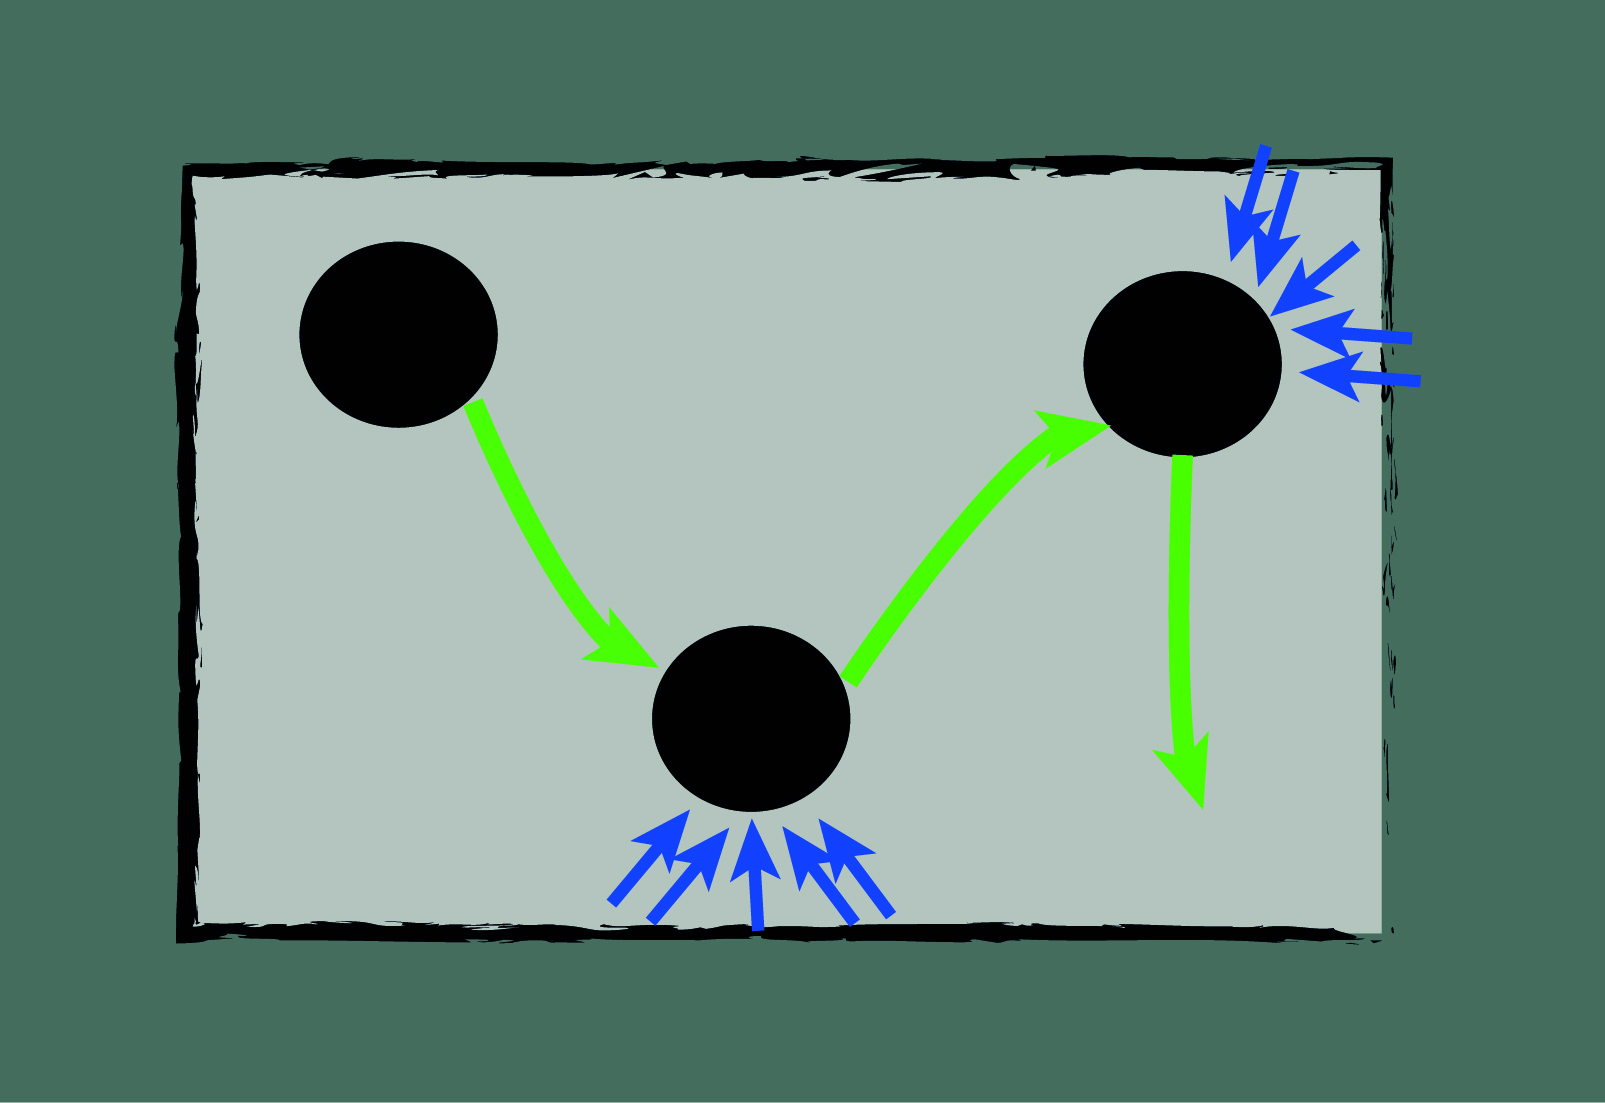
\includegraphics[width=.45\textwidth]{images/exploration2.jpg}}
        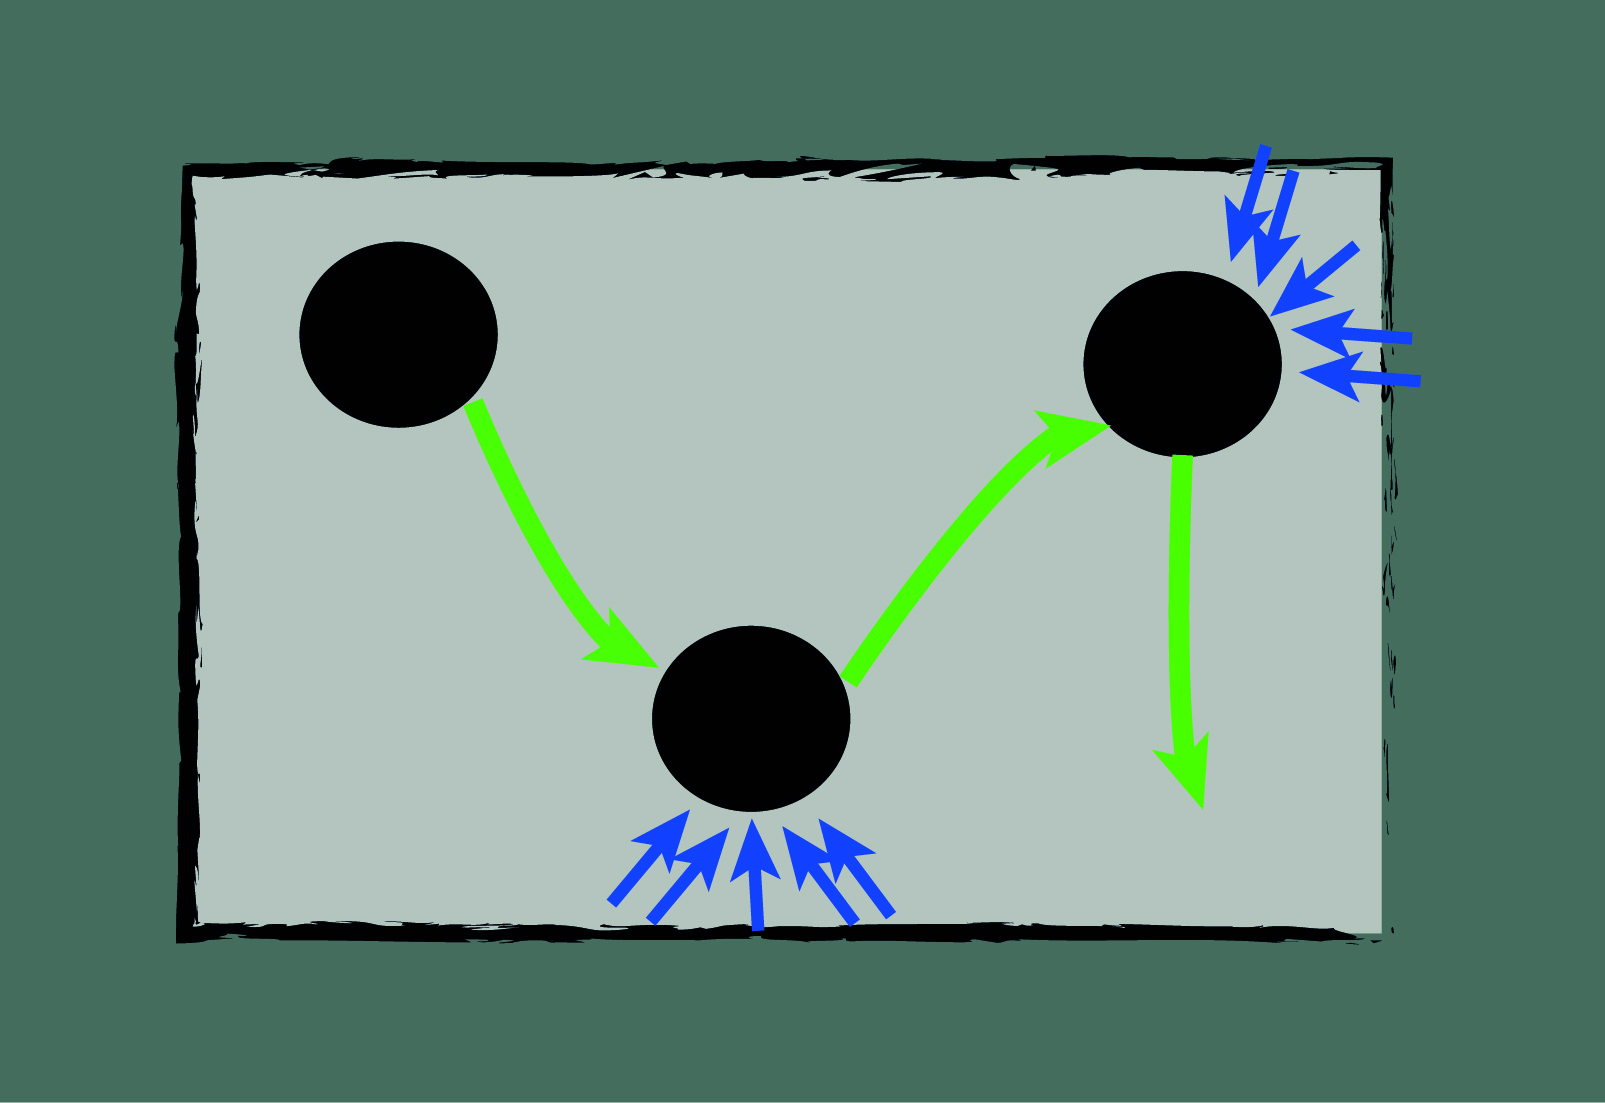
\includegraphics[width=.45\textwidth]{images/exploration2.jpg}\\
        (a)&(b)\\
        %\subfigure[]{\label{fig:etiquetaC}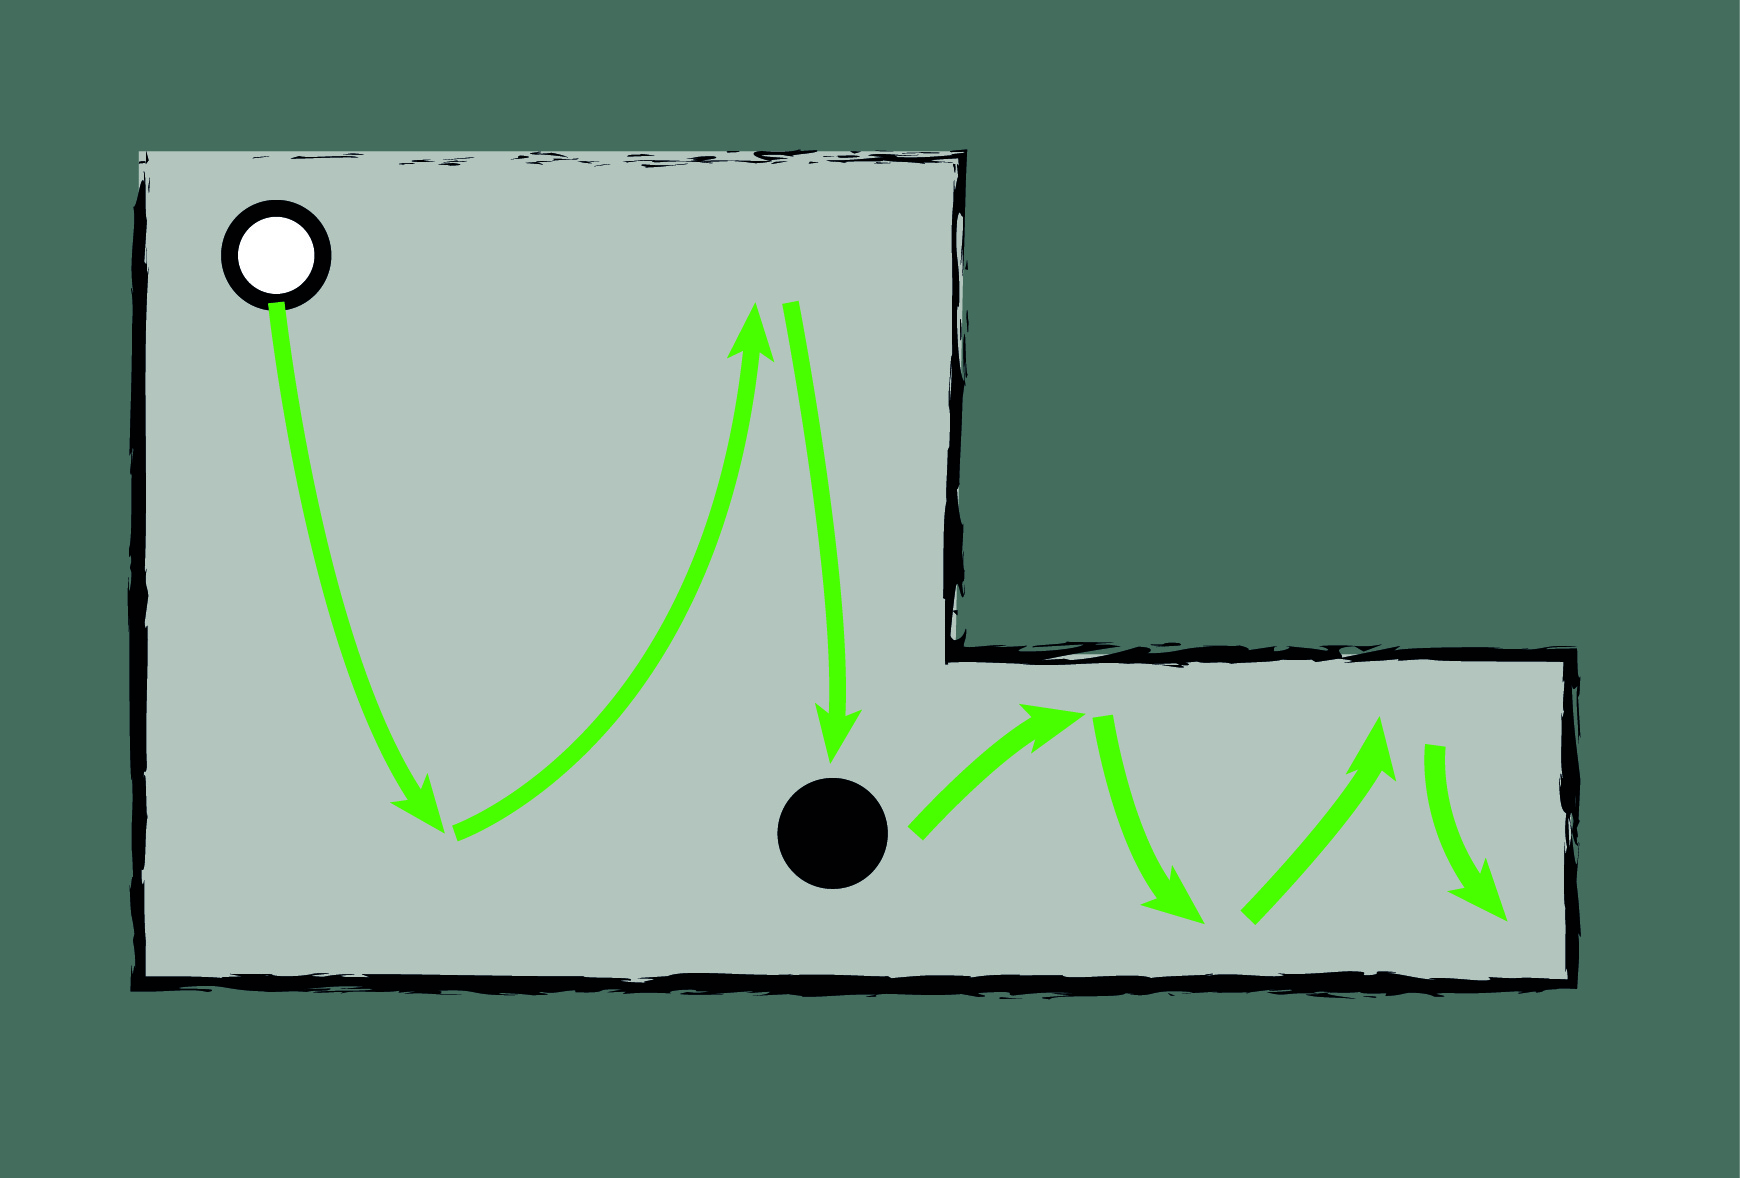
\includegraphics[width=.49\textwidth]{images/exploration3.jpg}}
        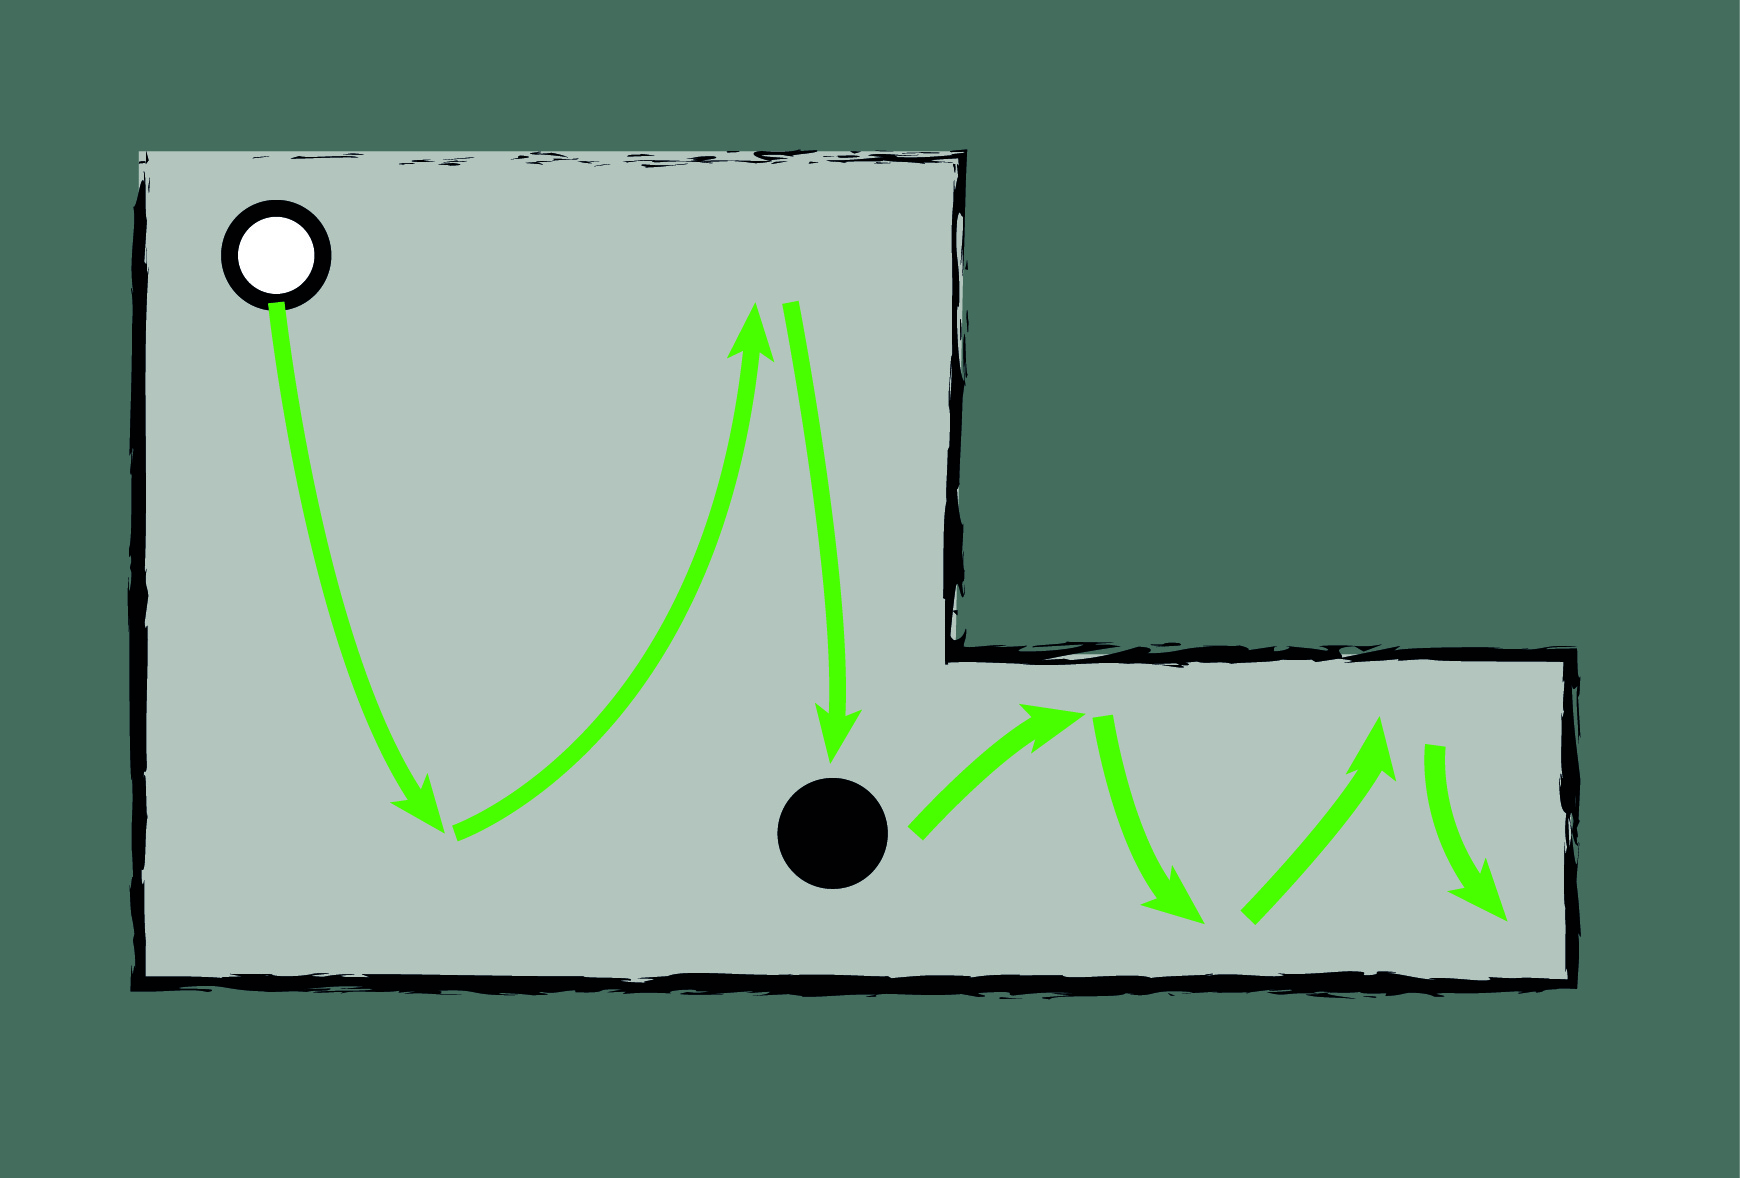
\includegraphics[width=.49\textwidth]{images/exploration3.jpg}&
        %\subfigure[]{\label{fig:etiquetaD}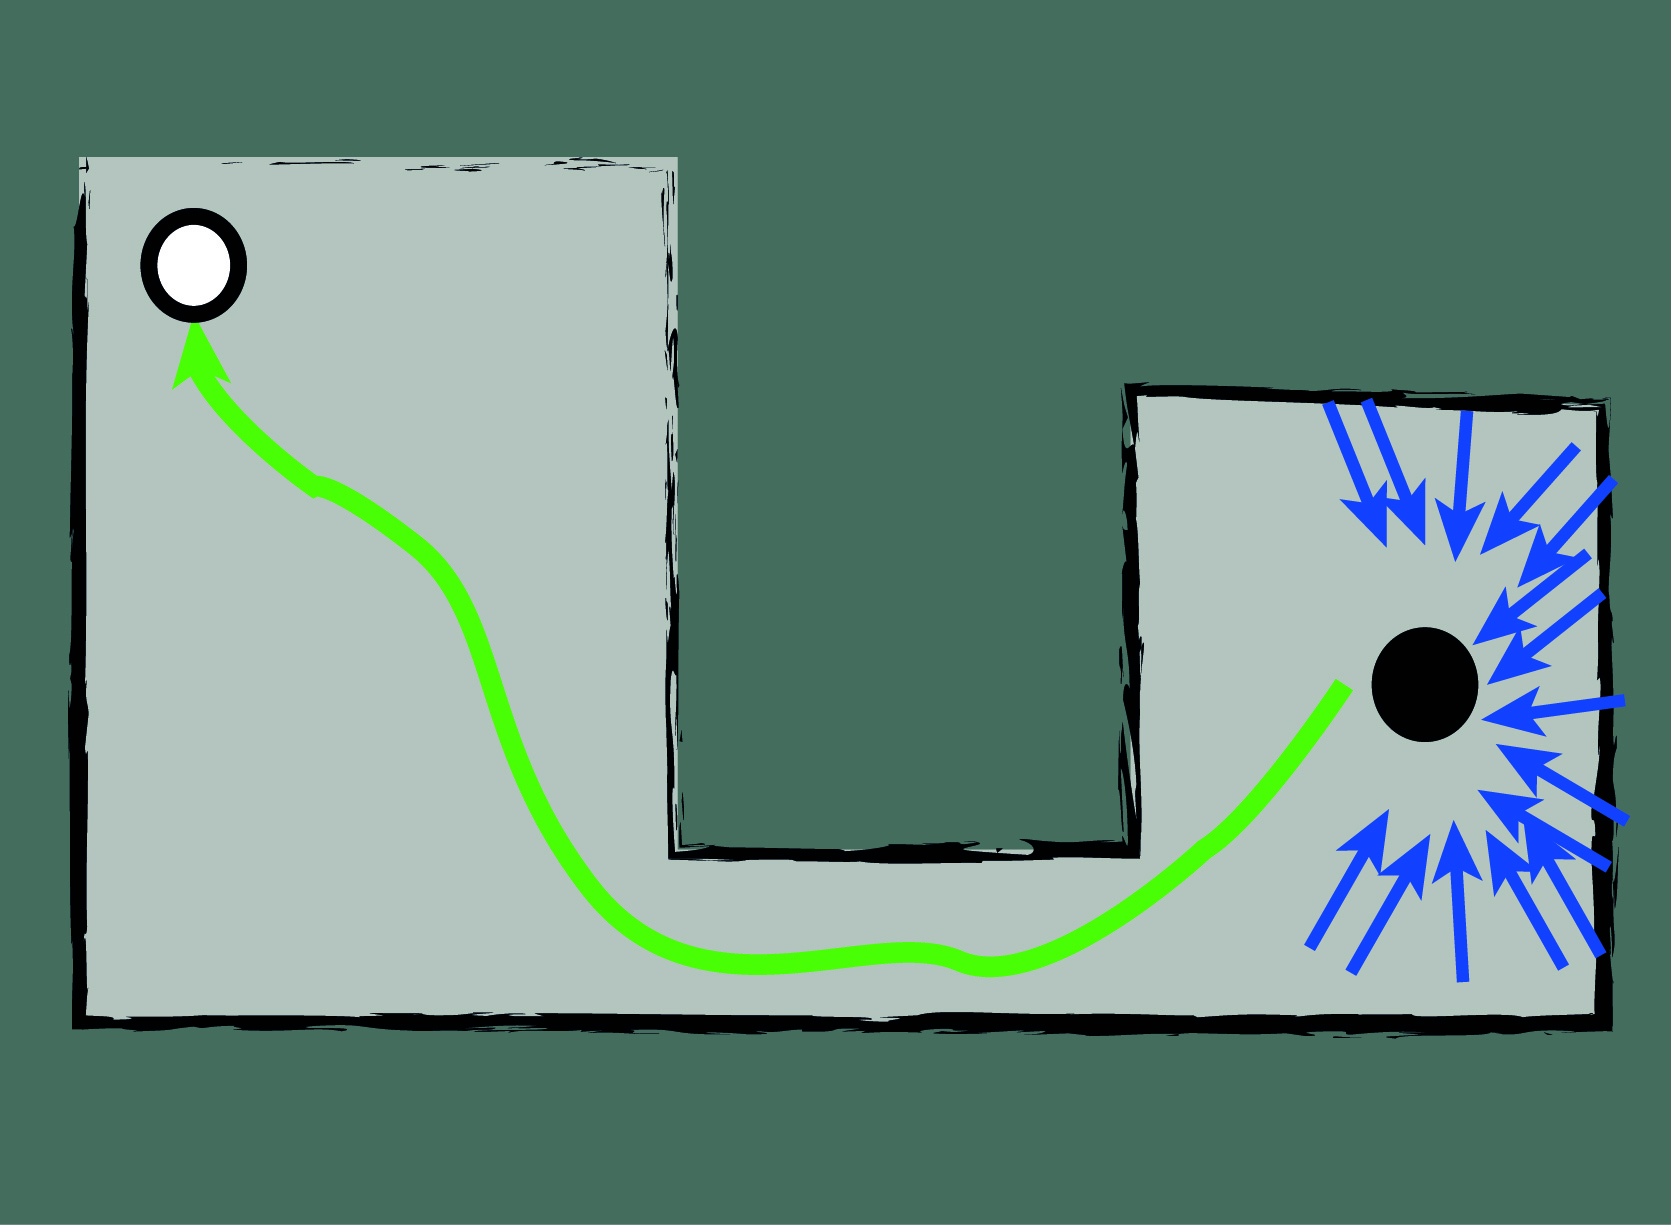
\includegraphics[width=.45\textwidth]{images/exploration4.jpg}}
        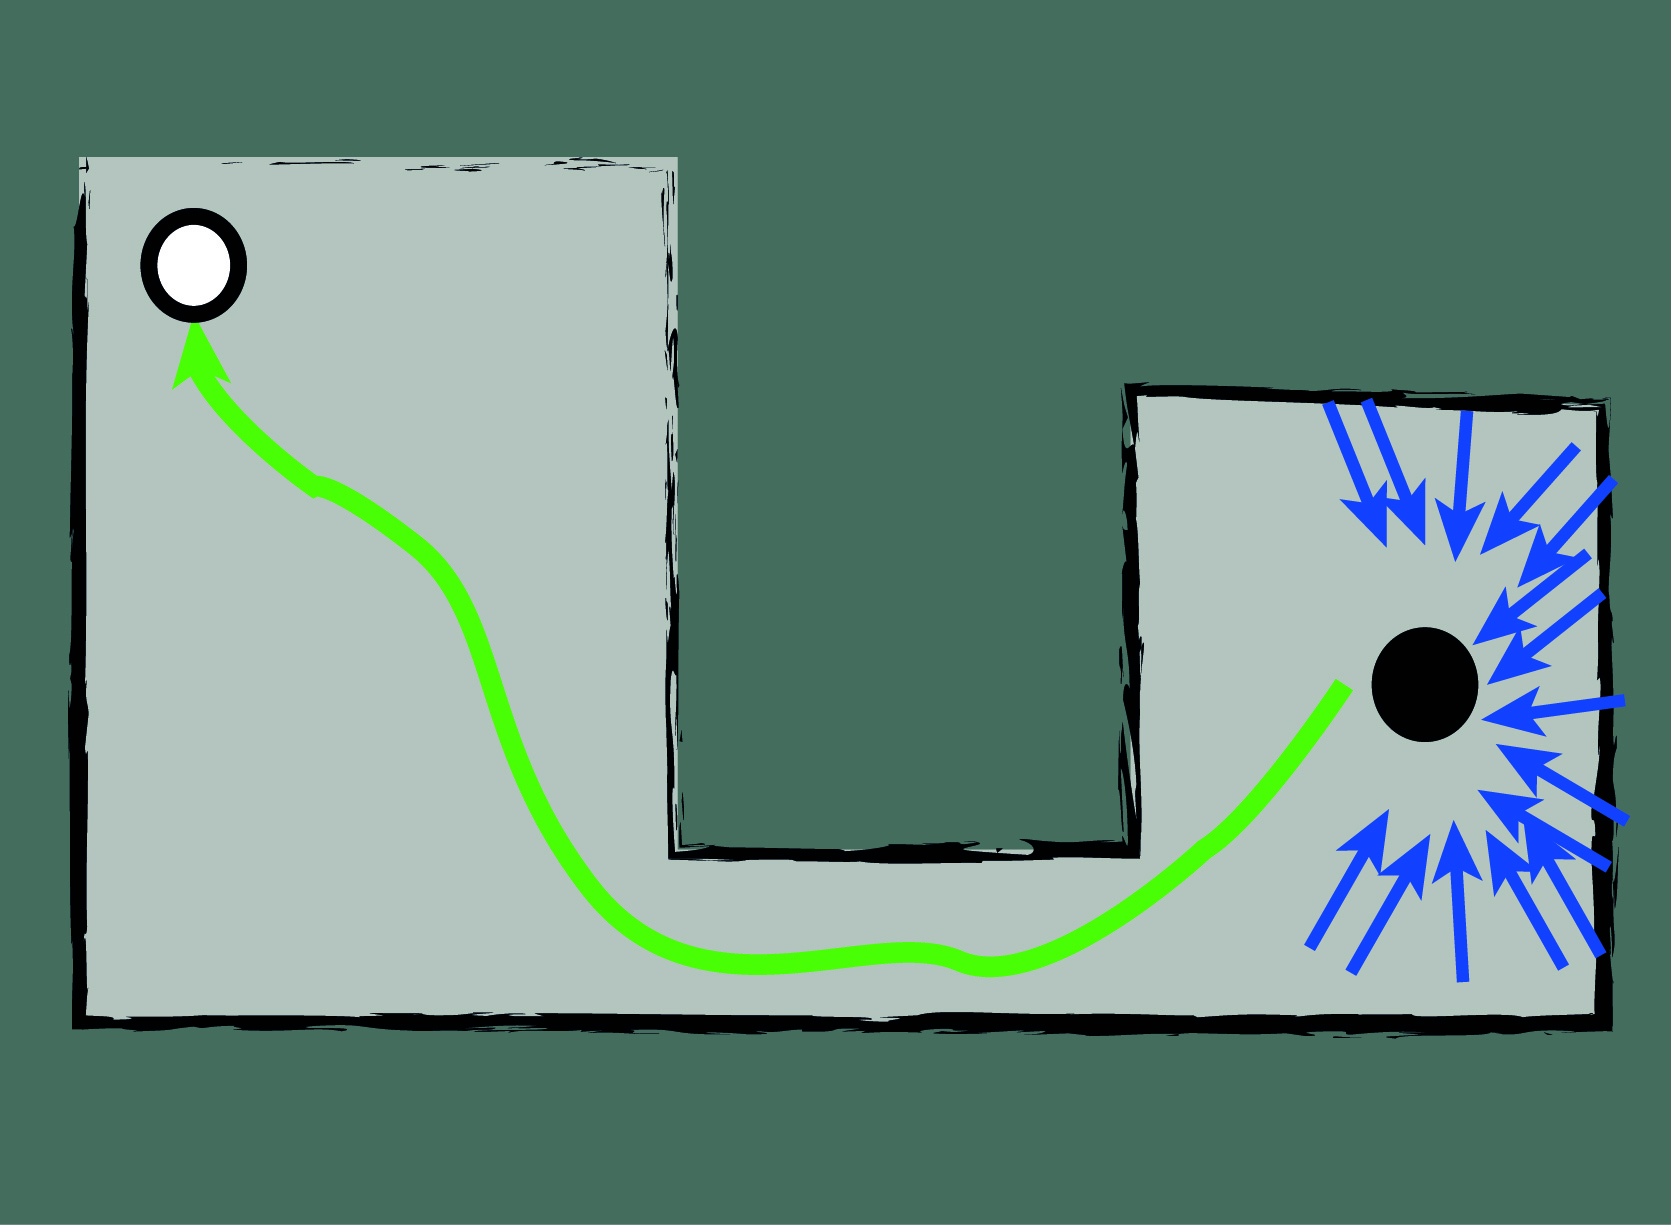
\includegraphics[width=.45\textwidth]{images/exploration4.jpg}\\
        (c)&(d)
    %\end{center}
    \end{tabular}
  \captionsetup{font=footnotesize}
    \caption{\label{f:SistemaAutonomo} En esta figura se muestra de forma gráfica las etapas del 
    sistema de autonomía del robot móvil. En (a) se muestra la etapa inicial que es el sensado de 
    las distancias, en (b) se muestra la evasión de obstáculos del robot móvil, en (c) se muestra
    las posiciones aleatorias por donde el robot tuvo que generar su trayectoria y en (d) se muestra
    como el robot ya no sabe por donde avanzar y regresa a su posición inicial.}
\end{figure}

La estructura del sistema de navegación autónoma del robot móvil diferencial se muestra en la
Figura \ref{fig:AutoSist}. Para que el robot móvil pueda localizarse dentro de un entorno 
desconocido, se utiliza el primer bloque que es el SLAM. Este algoritmo tiene como entradas 
los datos del sensor lidar y la odometría del robot ($x_{medido}, y_{medido}, \theta_{medido}$). El
algoritmo SLAM, como se menciono anteriormente, trabaja con filtros de partículas que ayudan 
a corregir la posición del robot dentro del ambiente que se va a desplazar. El SLAM tiene 
dos salidas, una es el mapa en dos dimensiones del lugar y la segunda salida es la localización
corregida del robot en el ambiente ($x_{corregido}, y_{corregido}, \theta_{corregido}$). El mapa
generado por el SLAM se da en tiempo real, lo cual permite que el robot pueda saber que lugares se
encuentra explorando.

%Para que el robot se localicé dentro de un ambiente desconocido, se utiliza el bloque del SLAM. 
%Este algoritmo tiene como entradas los datos del sensor lidar y de la odometría del robot 
%($x_{medido},y_{medido},\theta_{medido}$). El SLAM con los datos mencionados utilza filtros de 
%partículas y puede corregir la posición del robot dentro del ambiente desconocido. El 
%bloque de SLAM tiene como salidas el mapa en dos dimensiones del lugar y la localización del robot 
%corregido ($x_{corregido},y_{corregido},\theta_{corregido}$). El mapa en dos dimensiones permite
%visualizar el entorno, en tiempo real, que se esta explorando.

El segundo bloque de la estructura consiste en la etapa de exploración, este algoritmo tiene 
como entradas la localización del robot y el mapa en dos dimensiones dadas por el algoritmo
SLAM. Con la información de la localización del robot y el mapa en dos dimensiones la etapa 
comienza a generar posiciones deseadas de forma aleatoria dentro del ambiente, teniendo en 
consideración los obstáculos que se encuentran dentro de ella. 

El tercer bloque consiste en la navegación del robot móvil, esta navegación es realizada 
junto a los campos potenciales y el control de posición y orientación del robot móvil es 
utilizando el controlador polar. Estas teorías fueron explicadas en la sección 
\ref{sec:Campos Potenciales} y la sección \ref{sec:ControlPolar} respectivamente. Estas 
metodologías son empleadas para que el robot pueda generar su propia trayectoria evitando
los obstáculos y a su vez pueda tener un movimiento suave controlando su posición y 
orientación dentro del plano cartesiano. Este bloque necesita de la posición de los obstáculos
en el ambiente y de la posición deseada aleatoria, para que el robot, junto a los campos
potenciales pueda generar su propia trayectoria gracias a las fuerzas de atracción y de 
repulsión. Asimismo, el controlador polar ayuda a que el robot móvil pueda llegar exactamente
a la posición deseada dada de forma aleatoria. Finalmente, esta etapa tiene como salidas a la 
velocidad lineal y velocidad angular. Estas velocidades ingresan al robot móvil diferencial
haciendo que este se desplace dentro del ambiente donde se está explorando. El robot móvil 
como salida tiene los valores de la odometría, el cual ingresa a la etapa del SLAM haciendo que 
esta estructura se repita de forma iterativa.

La interacción autónoma del robot móvil dentro de un ambiente desconocido se puede ver en la 
Figura \ref{f:SistemaAutonomo}. En la Figura \ref{f:SistemaAutonomo}(a) se muestra la 
etapa inicial de la exploración del robot móvil, donde el robot móvil esta representado por 
el círculo de color negro y la figura geométrica de color rojo, representa las luces láser 
que emite el sensor lidar para realizar las mediciones. En esta etapa el sensor lidar comienza a 
tomar las primeras mediciones del ambiente desconocido, con esta información se comienza a 
construir el mapa en dos dimensiones del lugar. La Figura \ref{f:SistemaAutonomo}(b) se muestra 
el mapa originado por el SLAM, el cual tiene los colores característicos que representa
las zonas mencionadas en la sección \ref{sec:GMAPPING}. En esta figura se puede ver como el robot
móvil se desplaza dentro del ambiente. Cuando el robot recibe la información del mapa en dos 
dimensiones del algoritmo SLAM sabe que debe desplazarse por las zonas de color gris, en ese 
instante comienza a generar posiciones de forma aleatoria desplazándose hacia la izquierda. Este 
desplazamiento es originado por los campos potenciales explicado en la sección 
\ref{sec:Campos Potenciales}. Cuando el robot móvil se encuentra muy próximo a un obstáculo, en 
este caso una pared, los campos potenciales de repulsión evitan que el robot pueda chocarse contra
la pared u objeto. Estas fuerzas de repulsión están representados por flechas de color azul y la 
trayectoria del robot está representado por líneas de color verde, en la Figura 
\ref{f:SistemaAutonomo}(b). En la Figura \ref{f:SistemaAutonomo}(c) se muestra el desplazamiento 
que va realizando el robot móvil mientras va explorando el ambiente. Como se observa el 
desplazamiento del robot es hacia la derecha, luego hacia la izquierda esto se hace forma iterativa
y el cambio sucede cuando el robot se encuentra con un obstáculo. El robot cuando se encuentra 
con un obstáculo este rota en su propio eje y comienza a desplazarse alejándose del obstáculo. El robot 
sigue explorando el ambiente, ya que el mapa SLAM sigue mostrando zonas desconocidas. Finalmente, 
en la Figura \ref{f:SistemaAutonomo}(d) se muestra la situación cuando el robot ya no puede seguir 
explorando debido a que a sus alrededores se encuentran obstáculos que impiden el paso hacia las zonas
que aún falta por explorar, en este caso el robot rota en su propio eje y regresa a la posición 
donde comenzó a explorar ($\mayusx=0,\mayusy=0$).

%El bloque del campo potencial más control polar es la representación del algoritmo utilizado
%para la generación de trayectoria. Este algoritmo tiene como entradas los datos del sensor 
%lidar, la localización corregida del robot y la posición deseada. El algoritmo trabaja de forma 
%iterativa, tomando en consideración los obstáculos y la posición deseada. Para la exlporación del 
%robot dentro del ambiente desconocido, se toma posiciones deseadas de forma aleatoria que son
%entradas del algoritmo y a través de los campos potenciales el robot puede llegar hacia la posición 
%deseada. En el caso de que el robot mientras se va moviendo el sensor lidar detecte un obstáculo, 
%este enviará las posiciones del obstáculo y el algoritmo evitará que el robot se choque y a su vez
%pide una nueva posición deseada para que pueda crear una nueva trayectoria y seguir explorando el 
%ambiente. El controlador polar es utilizado para que el robot pueda moverse de forma suave en las 
%curvas que se forman al generar su propia trayectoria.

%Finalmente, el algoritmo de la generación de trayectoria tiene como salida la velocidad lineal y 
%velocidad angular que debe tener el robot para desplazarse dentro del ambiente que esta explorando. Todo 
%el sistema de navegación autónoma para el robot móvil se hace de forma iterativa hasta que el robot 
%termine de mapear todo el ambiente, una vez culminado el robot regresa hacia su posición inicial. El 
%sistema de navegación se puede ver en la figura \ref{fig:ArqSist}.


\section{Estructura del Sistema de Mapeo en Tres Dimensiones}
%\subsection{Estructura del Sistema de Mapeo en Tres Dimensiones}

\begin{figure}%[ht!]
	\centering \footnotesize
	\includegraphics[width=0.9\textwidth]{images/estructura_3d.png}
	\captionsetup{font=footnotesize}
	\caption{Estructura del sistema para la construcción del mapa en tres dimensiones, mientras el robot móvil
	se va desplazando.}
	\label{fig:Sist3D}
\end{figure}

En esta sección se explica de forma detallada las etapas por la cual esta conformada la estructura
del sistema para generar el mapa en tres dimensiones del ambiente. En la Figura \ref{fig:Sist3D} se 
muestra la estructura que genera los valores dentro de los tres ejes del plano cartesiano, mientras
el robot va explorando un ambiente.

El proceso comienza con la toma de mediciones de parte del sensor lidar, las mediciones que son 
obtenidas en tiempo real se encuentran en el formato de coordenadas polares ($r,\theta$). Estas 
medidas deben ser convertidas a coordenadas cartesianas, para encontrar las posiciones de los
objetos dentro del plano cartesiano bidimensional ($\mayusx_{L}, \mayusy_{L}$) y además conocer
las dimensiones que tiene el ambiente que se esta explorando.


%En esta parte del trabajo de tesis se muestra la estructura del sistema para realizar el
%mapa en tres dimensiones. La estructura se muestra en la figura \ref{fig:Sist3D}. Este 
%proceso comienza con las medidas que genera el sensor lidar, estas mediciones tienen
%que ser convertidas en posiciones dentro de las coordenadas cartesianas en dos dimensiones
%($X_{L}, Y_{L}$). La conversión a coordenadas polares permite conocer las posiciones de los 
%obstáculos dentro de un ambiente y asimismo conocer las dimensiones del entorno que se esta 
%explorando.
La segunda etapa de este proceso es hallar los valores de los ejes del plano cartesiano 
tridimensional, a partir de las transformaciones homogéneas. Para generar estos 
valores se necesita obtener los ángulos de rotación del motor paso a paso. Las matrices
de transformación homogénea y el principio de funcionamiento del sistema mecánico fueron
explicados en la sección \ref{sec:SistP3D}. Este sistema mecánico cuenta con dos sistemas
de referencia, uno es el sistema de referencia del sensor lidar y el segundo es el sistema
de referencia del motor paso a paso. Asimismo, el sistema mecánico genera movimientos de 
rotación y traslación; por ende, se utiliza transformaciones homogéneas ya que esto 
está compuesto por una matriz de rotación en el eje $\mayusy_{M}$ del motor paso a paso y
una matriz de traslación con un desplazamiento en el eje $\mayusz_{M}$ de dicho motor. La potencia
y la resolución angular del motor paso a paso permite que el sensor lidar tenga un ángulo de 
abertura de 176\grad~ el cual permite al sensor tener una amplia proyección en el eje $Z$ para
tomar mediciones. El resultado de las transformaciones homogéneas es una nube de puntos del
entorno explorado ($\mayusx, \mayusy, \mayusz$).

%Para obtener la nube de puntos, se necesita los ángulos de rotación del servomotor. El 
%servomotor hace rotar el sistema mecánico descrito y explicado en la sección 
%\ref{sec:SistP3D}. El sistema mecánico implementado tiene un movimiento de rotación y otro 
%de traslación. El sistema de referencia del sensor lidar se toma como el 
%sistema de referencia del servomotor. Por tal motivo se utiliza una matriz de transformación 
%homogénea, la cual esta compuesta por una matriz de rotación en el eje $Y_{S}$ del servomotor 
%y una matriz de traslación con un desplazamiento en el eje $Z_{S}$ del servomotor. El
%servomotor hace que el sensor lidar tenga un ángulo de abertura de 30\grad~ que permite
%hacer mediciones en el eje $Z$. El resultado de la multiplicación de las posiciones 
%($X_{L}, Y_{L}$) del sensor lidar con la matriz de transformación homogénea es
%una nube de puntos ($X_{M}, Y_{M}, Z_{M}$) del mapa del entorno.

Finalmente, la última etapa del sistema para generar el mapa en tres dimensiones es 
hacer que el mapa tenga correlación con el desplazamiento del robot dentro del 
ambiente. Para encontrar dicha correlación se debe obtener los valores de la odometría
del robot y estos deben ser sumados las posiciones del plano cartesiano tridimensional 
obtenido de las transformaciones homogéneas. La odometría del robot móvil diferencial 
es la estimación de la posición y orientación de este mientras se encuentra explorando 
el ambiente. La odometría del robot esta compuesta por tres valores 
($\mayusx_{R}, \mayusy_{R}, \theta_{R}$), estos valores son sumados a la nube de puntos
($\mayusx, \mayusy, \mayusz$). Cuando el robot realiza rotaciones en su propio eje ($\mayusz_{R}$) 
para el cambio de dirección en su trayectoria, esto debe ser considerado en la generación 
de la nube de puntos. Para este caso se utiliza el valor del ángulo de rotación del
robot móvil, obtenido de la odometría ($\theta_{R}$), dentro de una matriz de rotación del 
eje $\mayusz$. Esta matriz de rotación se multiplica con la nube de puntos obtenida 
anteriormente y el resultado de esto es el mapa en tres dimensiones del ambiente real 
explorado.



%El robot explora el entorno y a su vez va realizando el mapa en tres dimensiones de las zonas
%exploradas. El mapa debe tener correlación con la trayectoria que realiza el movimiento del 
%robot, para esto se debe sumar los valores de la odometría del robot móvil. La odometría del 
%robot es la estimación de la posición y orientación del robot mientras este se encuentra 
%navegando dentro de un ambiente. La odometría esta compuesta por tres valores ($X_{R}, Y_{R}, 
%\theta_{R}$). Para que el mapa pueda tener las posiciones con mayor precisión se suma los 
%valores de ($X_{R}, Y_{R}$) del robot a la nube de puntos del mapa tridimensional. Otra
%consideración en la construcción del mapa es la rotación del robot móvil al momento de 
%realizar giros en su propio eje $Z_{R}$. Para este caso se utiliza el valor del ángulo 
%de rotación ($\theta_{R}$) en una matriz de rotación del eje $Z$. Finalmente la nueva nube 
%de puntos multiplicado con la matriz de rotación en el eje $Z_{R}$ del robot, genera el mapa 
%en tres dimensiones de la zona explorada.
